%%
%%                     WHY ARE YOU READING THIS FILE?
%%
%% If you're looking for code examples for a particular typesetting
%% effect then you're looking in the wrong place.  The source to the
%% Visual LaTeX FAQ necessarily has to utilize a number of crude hacks
%% and is more often than not a demonstration of how *not* to achieve a
%% particular effect.  First, a lot of trickery is involved in wrapping
%% hyperlinks around typesetting examples: If you can't put something in
%% an \fbox and have it look right then you can't easily put a hyperlink
%% around it, either.  Second, some packages exhibit contradictory
%% functionality.  For example, parskip.sty sets the paragraph indent to
%% zero for all paragraphs while indentfirst.sty sets the paragraph
%% indent to a nonzero value for all paragraphs.  Clearly, a LaTeX file
%% can't meaningfully load both packages.
%%
%% The best way to get answers to typesetting questions is to browse
%% through the prebuilt visualFAQ.pdf file, click on hyperlinks of
%% interest, and learn from what the UK TeX FAQ has to say.
%%
\documentclass[twoside,letterpaper]{article}
\usepackage{etex}
\usepackage[marginparwidth=65pt, marginratio=1:1, tmargin=126pt, height=550pt, width=400pt]{geometry}
\usepackage{fancyhdr}
\usepackage{lastpage}
\usepackage{lettrine}
\usepackage{type1cm}
\usepackage{tabularx}
\usepackage{textcomp}
\usepackage{supertabular}
\let\STtopcaption=\topcaption
\let\topcaption=\relax
\usepackage{topcapt}
\usepackage{graphicx}
\usepackage{color}
\usepackage{layout}
\usepackage{setspace}
\usepackage{wrapfig}
\usepackage{amsmath}
\usepackage{amssymb}
\usepackage{mathrsfs}
\usepackage{texnames}
\usepackage{bold-extra}
\usepackage{eurosym}
\usepackage{slashbox}
\usepackage{multirow}
\usepackage{afterpage}
\usepackage{eso-pic}
\usepackage{calc}
\usepackage{multicol}
\usepackage{rotating}
\usepackage{fancyvrb}
\usepackage{makeidx}
\usepackage{framed}
\usepackage{cancel}
\usepackage{amsthm}
\usepackage[normalem]{ulem}
\usepackage{cooltooltips}
\usepackage[bookmarksopen,pdfpagemode=UseNone]{hyperref}

% Specify the document's metadata.
\hypersetup{%
  pdftitle={The Visual LaTeX FAQ},
  pdfauthor={Scott Pakin, scott+vfaq@pakin.org},
  pdfsubject={Answers to frequently asked questions regarding LaTeX},
  pdfkeywords={%
    LaTeX, tables, figures, typesetting, spacing, spaces, hyphenation,
    sections, titles, verbatim, fonts, symbols, characters, floats,
    bibliography, BibTeX, page numbers, footnotes, columns,
    mathematics, captions, references, citations, alignment
  }
}

% Discourage the user from compiling this document himself.
\makeatletter
\@ifundefined{vlfpoweruser}{%
  \GenericError
    {(visualFAQ)\@spaces\@spaces}
    {visualFAQ Error: You really don't want to build the Visual LaTeX FAQ}
    {See the README file in this directory for an explanation.}
    {The visualFAQ.pdf file on CTAN has been postprocessed to\MessageBreak
     include page thumbnails and to support "Fast Web View"\MessageBreak
     (a.k.a. Linearized PDF).  Rebuilding the PDF will lose that\MessageBreak
     metadata.  Changes to the document, including formatting\MessageBreak
     changes, are also not recommended.  Because of the extensive\MessageBreak
     use of unbreakable TeX boxes the document is very sensitive\MessageBreak
     to layout.  Any change is likely to cause ugly slabs of\MessageBreak
     inter- and intraparagraph whitespace to appear throughout\MessageBreak
     the document.}
  \begin{document}
    \VerbatimInput[fontsize=\small]{README.TXT}
  \end{document}
}{}
\makeatother

% Define a shortcut for hyperlinks to the UK TeX FAQ.
\newsavebox{\faqbox}
\DeclareRobustCommand{\faq}[3]{%
  \begin{lrbox}{\faqbox}#3\end{lrbox}%
  \cooltooltip[0 1 0]{FAQ}{#2}%
    {http://www.tex.ac.uk/cgi-bin/texfaq2html?label=#1}%
    {http://www.tex.ac.uk/.../#1}%
    {\usebox{\faqbox}}%
}

% Define a variation of \faq that indicates that the user wants certain
% formatting _not_ to occur.
\DeclareRobustCommand{\antifaq}[3]{%
  \begin{lrbox}{\faqbox}#3\end{lrbox}%
  \cooltooltip[1 0 0]{FAQ}{#2}%
    {http://www.tex.ac.uk/cgi-bin/texfaq2html?label=#1}%
    {http://www.tex.ac.uk/.../#1}%
    {\usebox{\faqbox}}%
}

% Define the paragraph indent and a command to force that indent.
\newlength{\defaultparindent}
\setlength{\defaultparindent}{15pt}
\setlength{\parindent}{\defaultparindent}

% Center a graphic on the page.
\newsavebox{\graphicbox}
\newlength{\graphicx}
\newlength{\graphicy}
\newcommand{\centergraphic}[3][!]{%
  \savebox{\graphicbox}{\includegraphics{#3}}%
  \setlength{\graphicx}{(\paperwidth-\wd\graphicbox)/2}
  \setlength{\graphicy}{(\paperheight-\ht\graphicbox)/2}
  \ifx#1!
    \AddToShipoutPicture*{%
      \put(\LenToUnit{\graphicx},\LenToUnit{\graphicy}){\usebox{\graphicbox}}
    }%
  \else
    \AddToShipoutPicture*{%
      \put(\LenToUnit{\graphicx},\LenToUnit{\graphicy}){\faq{#1}{#2}{\usebox{\graphicbox}}}
    }%
  \fi
}

% Specify the float parameters from "Moving tables and figures in LaTeX".
\renewcommand{\topfraction}{.85}
\renewcommand{\bottomfraction}{.7}
\renewcommand{\textfraction}{.15}
\renewcommand{\floatpagefraction}{.66}
\renewcommand{\dbltopfraction}{.66}
\renewcommand{\dblfloatpagefraction}{.66}
\setcounter{topnumber}{9}
\setcounter{bottomnumber}{9}
\setcounter{totalnumber}{20}
\setcounter{dbltopnumber}{9}

% Provide a fake \cite command to help showcase label=backref.
\newcommand{\fakecite}[1]{[\hypergetref{cite:backref}\label{#1}]}

% Define a \nolinkfootnotemark as a non-hyperlinked \footnotemark.
\makeatletter
\let\nolinkfootnotemark=\H@@footnotemark
\makeatother

% FAQ: "Alternative head- and footlines in LaTeX"
% FAQ: "Page numbering '<n> of <m>'"
% FAQ: "How many pages are there in my document?"
\fancypagestyle{fancybasic}{%
  \fancyhf{}
  \fancyhead[LO,RE]{%
    \faq{fancyhdr}{"Alternative head- and footlines in LaTeX"}{%
      \usefont{T1}{pzc}{m}{it}\leftmark}}
  \fancyhead[LE,RO]{%
    \faq{fancyhdr}{"Alternative head- and footlines in LaTeX"}{%
      \usefont{T1}{pzc}{m}{it}\rightmark}}
  \cfoot{%
    \faq{nofm+howmanypp}%
      {"Page numbering '<n> of <m>'" and "How many pages are there in my document?"}%
      {Page~\thepage\ of~\pageref*{LastPage}}\strut}
}
\pagestyle{fancybasic}

% FAQ: "Page numbering by chapter"
\newcounter{sectionfirstpage}
\newcounter{pageofsection}
\fancypagestyle{fancyaltpagenum}{%
  \cfoot{%
    \setcounter{pageofsection}{\thepage-\thesectionfirstpage+1}%
    \faq{pagebychap}%
      {"Page numbering by chapter"}%
      {\Roman{section}--\thepageofsection\strut}%
  }%
}

% Define verbatim left and right braces, a verbatim backslash, and a
% verbatim space for use in popup messages.
\bgroup
\catcode`\<=1
\catcode`\>=2
\catcode`\{=11
\catcode`\}=11
\gdef\verblbrace<{>
\gdef\verbrbrace<}>
\catcode`\|=0
\catcode`\\=11
|gdef|verbbslash<\>
|egroup
\let\verbspace=\space

% FAQ: "\pagestyle{empty} on first page in LaTeX"
% FAQ: "How to get rid of page numbers"
\fancypagestyle{fancyplain}{%
  \fancyhf{}
  \renewcommand{\headrulewidth}{0pt}
  \cfoot{%
    \faq{ps@empty+nopageno}%
      {"\verbbslash\verbbslash
       pagestyle\verblbrace empty\verbrbrace\verbspace on first page in LaTeX"
       and "How to get rid of page numbers"}%
      {\qquad\strut}%
  }%
}

% Define the same style as fancybasic but without the hyperlinks.
\fancypagestyle{fancynohyper}{%
  \fancyhf{}
  \fancyhead[LO,RE]{\usefont{T1}{pzc}{m}{it}\leftmark}
  \fancyhead[LE,RO]{\usefont{T1}{pzc}{m}{it}\rightmark}
  \cfoot{Page~\thepage\ of~\pageref*{LastPage}}
}

% For framed.sty, define a set of macros needed to illustrate the way a
% box can be broken across pages.
\newsavebox{\brokenbox}
\newlength{\boxlower}
\def\partialframebox[#1#2]#3{%
  \setlength{\boxlower}{\fboxrule+\fboxsep+\dp\brokenbox}%
  \faq{breakbox}{"Breaking boxes of text"}{%
    \setlength{\fboxrule}{3pt}%
    \lower\boxlower\hbox{%
      \vbox{%
        \ifx#1t\hrule height \fboxrule \fi
        \hbox{%
          \vrule width \fboxrule
          #3%
          \vbox{%
            \vskip\fboxsep
            \box\brokenbox
            \vskip\fboxsep}%
          #3%
          \vrule width \fboxrule}%
          \if#2b\hrule height \fboxrule \fi
      }%
    }%
  }%
}
\definecolor{lightgray}{rgb}{0.85, 0.85, 0.9}
\newcommand{\topthenbottomframe}[1]{%
  \savebox{\brokenbox}{\colorbox{lightgray}{#1}}%
  \ifnum\currentframe<5
    \partialframebox[t-]{\kern\fboxsep}%
  \else
    \partialframebox[-b]{\kern\fboxsep}%
  \fi
  \global\advance\currentframe by 1
}
\makeatletter
\newcount\currentframe
\newenvironment{brokenfaqbox}{%
  \global\currentframe=0\relax
  \let\FrameCommand=\topthenbottomframe
  \MakeFramed{\advance\hsize-\width\FrameRestore}%
}{%
  \endMakeFramed
}
\makeatother

% Define a new log-like function.
\DeclareMathOperator*{\loremop}{lorem}

% Define a larger-than-normal set of math font sizes.
\DeclareMathSizes{10.1}{18}{14}{12}

% We use the following as our generic graphic.
\newsavebox{\logobox}
\savebox{\logobox}{
\includegraphics[height=3cm]{lorem-ipsum-logo}}

% We use the text "Where can I find the symbol for ..." in a number of places.
\newcommand*{\wheresym}{"Where can I find the symbol for ..."}

% Draw slightly bolder hyperlink borders than the default.
\setlength{\fboxrule}{1.5pt}

%%%%%%%%%%%%%%%%%%%%%%%%%%%%%%%%%%%%%%%%%%%%%%%%%%%%%%%%%%%%%%%%%%%%%%%%%%%

\begin{document}
\thispagestyle{fancyplain}
\sloppy
\raggedbottom

% Give the user the ability to disable popups.
\newsavebox{\togglebox}
\savebox{\togglebox}{%
  \fcolorbox{red}{yellow}{%
    \small
    \begin{tabular}[t]{l}
      This document uses PDF popups, which may cause problems for some PDF \\
      viewers. Click here to enable/disable the popup mechanism document-wide.
    \end{tabular}%
  }%
}
\AddToShipoutPicture*{%
  \AtPageUpperLeft{%
    \put(0,\LenToUnit{-\ht\togglebox}){%
      \cooltooltiptoggle{\usebox{\togglebox}}%
    }%
  }%
}

% FAQ: "The style of document titles"
\noindent
\faq{titlsty}{"The style of document titles"}{%
  \begin{minipage}{\linewidth}
  \rule{\linewidth}{3pt}\par
  \vspace*{4ex}%
  \noindent{\fontsize{36}{43}\usefont{OT1}{phv}{b}{n}The Visual \LaTeX{} FAQ}
  \vspace*{4ex}
  \begin{flushright}
  \large\usefont{OT1}{pnc}{m}{n}
  Scott Pakin\par
  {\small\textit{scott+vfaq@pakin.org}}\par
  \vspace*{3ex}
  \today
  \end{flushright}
  \rule{\linewidth}{3pt}
  \end{minipage}
}
\vspace{1cm}

% FAQ: "1-column abstract in 2-column document"
\noindent
\faq{onecolabs}{"1-column abstract in 2-column document"}{%
\begin{minipage}{\linewidth}
\begin{abstract}\strut
  This document provides an experimental new ``search'' interface to
  UK \TeX\ FAQ (\nolinkurl{http://www.tex.ac.uk}).  Rather than
  require the user to formulate a query, it merely presents examples
  of customized \LaTeX{} formatting---and formatting
  problems---encased in live hyperlinks (green or red, as appropriate)
  to appropriate pages in the FAQ\@.  The goal is to facilitate
  finding answers to \LaTeX-related queries which are difficult to
  formulate textually but easy to recognize visually.

  In short: If you want to learn how something in this document was
  formatted or why it came out misformatted, just click on it.\strut
\end{abstract}
\end{minipage}
}
\bigskip

% FAQ: "Changing the margins in LaTeX"
\makeatletter
\newsavebox{\marginbox}
\begin{lrbox}{\marginbox}
\begin{minipage}{\linewidth}
  \centering
  \let\newpage=\relax
  \@twosidefalse
  \vspace*{\baselineskip}%
  \layout
  \rule{0pt}{7\baselineskip}%
\end{minipage}
\end{lrbox}
\makeatother
\begin{figure*}[tbp]
  \faq{changemargin}{"Changing the margins in LaTeX"}{\usebox{\marginbox}}
\end{figure*}

\begin{multicols}{2}
\section{Magna condimentum}
\thispagestyle{fancyplain}   % Why can't this go earlier?

% FAQ: "Big letters at the start of a paragraph"
\lettrine[lines=3]{\faq{dropping}{"Big letters at the start of a
paragraph"}{L}}{orem} ipsum dolor sit amet, consectetuer adipiscing
elit. Ut ligula nisl, euismod at, sagittis dapibus, dapibus non,
velit. Curabitur mauris nibh, consequat iaculis, suscipit id,
ullamcorper eu, eros.  \AE{}nean eget langilla metus non mi.  Vivamus
facilisis laoreet massa. Fusce nunc mi, rutrum et, cursus sed, congue
ac, velit.

% FAQ: "Changing the space between letters"
% FAQ: "Realistic quotes for verbatim listings"
\newcommand*{\upquotfaq}[1]{%
  \faq{upquot}{"Realistic quotes for verbatim listings"}{#1}%
}
Quisque eu lacus. Vivamus vel natoque fames
\faq{letterspace}{"Changing the space between
letters"}{\textsc{a\,d\,i\,p\,i\,s\,c\,i\,n\,g}} nulla. Fusce nec urna
eget justo consequat convallis. Vestibulum diam. Cras ac felis eget
quam venenatis fermentum.  Volutpat non, egestas sit amet, tincidunt
vit\ae{}, metus. Nunc enim nulla, luctus nec, bibendum in,
sollicitudin sit amet, tortor. Proin id ipsum congue hendrerit mattis,
``\texttt{echo Justo \upquotfaq{\textquotesingle}at
enim\upquotfaq{\textquotesingle}\upquotfaq{\textasciigrave}expr 2 +
2\upquotfaq{\textasciigrave}}''.  Fusce turpis, Pr\ae{}sent malesuada,
lorem sem sagittis est, vit\ae{} laoreet odio arcu auctor
consectetuer.

% FAQ: "What's the name of this file"
% FAQ: "Printing the time"
In vehicula sagittis nisl. M\ae{}cenas malesuada feugiat eros. Nulla
facilisis accumsan quam. Nulla id nunc \faq{filename}{"What's the name
of this file"}{\strut\texttt{\jobname.tex}} duis \faq{time}{"Printing
the time"}{\strut\today~10:51pm} facilisis tristique
lectus. Vestibulum ante ipsum primis in faucibus orci luctus et
ultrices posuere cubilia cur\ae{}; Vivamus dictum nibh vit\ae{} mi.

% FAQ: "How to use the underscore character"
% FAQ: "Typesetting the Euro sign"
% FAQ: "How to get copyright, trademark, etc."
% FAQ: "Where can I find the symbol for ..."
At vero eos et accusam et fabulas deleni \faq{underscore}{"How to use
the underscore character"}{\texttt{justo\_duo\_dolores()}} et ea
rebum. Stet clita kasd gubergren, no sea takimata
\faq{euro+symbols}{"Typesetting the Euro sign" and
\wheresym}{\officialeuro\strut}21.50 sanctus est.  At quo verear
vocibus, delenit blandit vim ex, et noster percipit eam. Duo hinc
Platonem Maluisset\faq{tradesyms+symbols}{"How to get copyright,
trademark, etc." and \wheresym}{\textsuperscript{\textregistered}} eu,
mel legendos vituperatoribus te. Duo ea dolor libris molestie,
Cotidieque~\faq{tradesyms+symbols}{"How to get copyright, trademark,
etc." and \wheresym}{\textcopyright}~\the\year\ alia Utinam Aliquam
ut vel no laudem eirmod virtute.
\end{multicols}

\section{Morbi tincidunt lacus}

% FAQ: "Typesetting epigraphs"
\begin{flushright}
\faq{epigraph}{"Typesetting epigraphs"}{%
\begin{minipage}{0.5\linewidth}
\small
\textit{Fusce dignissim, pede ac euismod fermentum, eros magna dapibus
leo, nec sodales libero urna tincidunt tellus.}

\hfill---\,\textsc{Cras Magna}
\end{minipage}}
\end{flushright}

\medskip

% FAQ: "Why doesn't \verb work within ...?"
\newsavebox{\verbbox}
\begin{lrbox}{\verbbox}
\verb.`~!@#$%^&*()-_+=[]{}|\;:'<>.
\end{lrbox}
%$
\noindent
Quam vestibulum, euismod taciti semper donec adipiscing. Fusce commodo
mus nonummy proin lacus cur\ae{} lacus donec nisl malesuada bibendum
sem senectus euismod amet. Fermentum massa, quisque
porttitor.\footnote{Nunc commodo \faq{verbwithin}{"Why doesn't
\verbbslash verb work within
...?"}{\usebox{\verbbox}} velit sed augue.}

Dui fermentum quisque commodo consectetuer torquent ligula. Tristique
id. Dignissim non ac, posuere euismod.  In eu quam etiam urna. Duis
rhoncus viverra sapien.  Rutrum congue adipiscing posuere massa
natoque.


\subsection{Vehicula enim}

% FAQ: "Typesetting URLs"
Nunc nonummy sapien nec quam. Phasellus eros est, eleifend vel,
aliquam id, tempor \faq{setURL}{"Typesetting
URLs"}{\nolinkurl{http://this.is/~my/typeset/URL.html}} iaculis,
felis.  M\ae{}cenas ultrices, velit auctor lacinia hendrerit, nisl
magna consectetuer ipsum, vel tincidunt neque quam at purus.

\subsubsection{Phasellus orci quam}

Aliquam quis justo vel lectus rhoncus placerat.  Elementum
lobortis. Torquent dolor integer commodo sapien tristique dictum non
pr\ae{}sent lorem ornare, sapien dis.

% FAQ: "Quality of PDF from PostScript"
\smallskip\noindent
\antifaq{dvips-pdf}{"Quality of PDF from PostScript"}{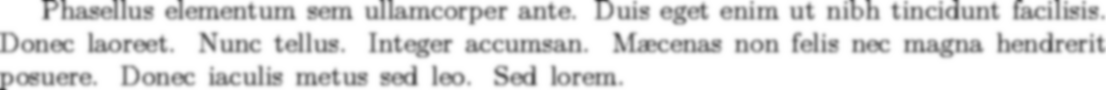
\includegraphics{fuzzytext}}

Amet magna id \ae{}nean. Phasellus rutrum montes placerat sed elit,
amet sollicitudin metus et lacinia. Habitasse aliquet. Cras tristique
nulla vit\ae{} nisl.  Vivamus sem eros, sollicitudin at, volutpat at,
pretium ut, mi. Cras erat. Vivamus sagittis. Phasellus id elit non
massa auctor tempor.

% FAQ: "How to create a \subsubsubsection"
\bigskip
\noindent
\faq{subsubsub}{"How to create a \verbbslash\verbbslash subsubsubsection"}{%
  \normalfont\itshape
  2.1.1.1\quad Suspendisse pulvinar}
\bigskip

\noindent
Nam vestibulum risus ut est. Sed semper, tellus lobortis tempor
euismod, nunc massa sagittis enim, a accumsan sapien enim ut
nisi. Cras rutrum dignissim libero.  Nulla consequat risus non nisl.


\section{Fusce dignissim}

% FAQ: "Indent after section headings"
\faq{secindent}{"Indent after section headings"}{\hspace*{2em}\strut}%
\AE{}nean tincidunt ipsum tincidunt felis. Class aptent taciti
sociosqu ad litora torquent per conubia nostra, per inceptos
hymen\ae{}os. Nunc auctor. Etiam faucibus nulla eu dolor.  Sociis
tristique neque suspendisse nonummy mi metus congue class \AE{}nean
curabitur fames habitant ullamcorper interdum lobortis.

\subsection{Vestibulum ante ipsum primis}

\begingroup
\setlength{\parindent}{0pt}
\setlength{\parskip}{\baselineskip}

% FAQ: "Zero paragraph indent"
Pr\ae{}sent varius vehicula enim. Proin nec massa. Vivamus lorem pede,
rhoncus et, mollis ut, laoreet nec, justo. Nullam vel
mauris. \AE{}nean quis libero.  Sed tempus lobortis ante. Duis euismod
condimentum sapien.\hfill\mbox{}\linebreak
%
\faq{parskip}{"Zero paragraph indent"}{\hspace*{\linewidth}\strut}\linebreak
%
Cum sociis natoque penatibus et magnis dis parturient montes, nascetur
ridiculus mus. Pellentesque eu massa. Duis consectetuer elit a
risus. Proin malesuada, nisl sed mattis fringilla, est lorem varius
augue, eget consectetuer lorem urna adipiscing nibh.\hfill\mbox{}\linebreak
%
\faq{parskip}{"Zero paragraph indent"}{\hspace*{\linewidth}\strut}\linebreak
%
Class aptent taciti sociosqu ad litora torquent per conubia nostra,
per inceptos hymen\ae{}os. In vehicula ornare dui. Fusce eget justo
sit amet nulla molestie volutpat. Pellentesque eleifend eros posuere
nibh. Nunc hendrerit, leo semper mattis dapibus, enim nibh blandit
sem, nec pharetra nisl metus vehicula sapien.
\endgroup


% FAQ: "The style of section headings"
\bigskip
\refstepcounter{section}
\begin{center}
\faq{secthead}{"The style of section headings"}{%
  \begin{tabular}{@{}c@{}}
    \hline
    \sffamily\Large\strut\thesection.\quad Donec purus \\
    \hline
  \end{tabular}
}
\end{center}
\sectionmark{Donec purus}
\phantomsection
\addcontentsline{toc}{section}{Donec purus}

% FAQ: "Page numbering by chapter"
\setcounter{sectionfirstpage}{\thepage}
\pagestyle{fancyaltpagenum}

% FAQ: "Sorting and compressing citations"
\noindent
Mauris mi libero, sollicitudin nec, sollicitudin ac, facilisis vel,
tellus. Sed dapibus semper dolor. Morbi tincidunt lacus et
mauris~\faq{citesort}{"Sorting and compressing
citations"}{[1--3,6]}. Mauris id dolor vel lacus aliquam egestas. Ut
vel nulla vel purus fermentum ornare. Phasellus
velit~\fakecite{backbackref1}. Aliquam suscipit ante nec felis. Sed
nonummy mauris eget neque. Fusce dignissim, pede ac euismod fermentum,
eros magna dapibus leo, nec sodales libero urna tincidunt tellus.

% FAQ: "Using PostScript fonts with TeX"
\noindent
\faq{usepsfont}{"Using PostScript fonts with TeX"}{%
\begin{minipage}{\linewidth}
\setlength{\parindent}{\defaultparindent}\strut
{\usefont{T1}{ptm}{m}{n} Velit viris euismod sit in.}
{\usefont{T1}{phv}{m}{n} Ut vituperatoribus prodesset eam, an quo
ferri oblique.}  {\usefont{T1}{pcr}{m}{n} Stet docendi vix id, sale
torquatos an mel.}  {\usefont{T1}{pag}{m}{n} No pro dicunt mollis, quo
platonem prodesset te, usu elit interesset in.}
{\usefont{T1}{pbk}{m}{n} At veri dicunt electram vis, ea sea nemore
denique omnesque.}  {\usefont{T1}{pzc}{m}{n} Quo idque principes
hendrerit et.}  {\usefont{T1}{ppl}{m}{n} Has ut nostro iudicabit
intellegam.}  {\usefont{T1}{pnc}{m}{n} Ex nihil aperiri per.}
{\usefont{T1}{bch}{m}{n} Iudico meliore at sed.}\strut
\end{minipage}%
}

% FAQ: "Top-aligning imported graphics"
\begin{figure}[tp]
  \faq{topgraph}{"Top-aligning imported graphics"}{%
    \begin{tabular*}{\linewidth}{l@{\extracolsep{\fill}}c@{\extracolsep{\fill}}c@{\extracolsep{\fill}}l}
      &
      \vtop{%
        \vskip0pt
        \hbox{%
          \color{blue}%
          \rule[-1ex]{1cm}{1ex}%
          \rule[-1cm]{1ex}{1cm}%
          \rule[-1ex]{1cm}{1ex}%
        }%
      } &
      \vtop{%
        \vskip0pt
        \hbox{%
          \color{blue}%
          \rule[-1ex]{1cm}{1ex}%
          \rule[-3cm]{1ex}{3cm}%
          \rule[-1ex]{1cm}{1ex}%
        }%
      } \\
    ~\\[1ex]
    & (a)~Sollicitudin ac & (b)~Fusce ut massa \\
  \end{tabular*}%
  }
  % FAQ: "The style of captions"
  \makeatletter
  \renewcommand{\fnum@figure}{%
    \faq{captsty}{"The style of captions"}{\textbf{Fig.~\thefigure}}}
  \makeatother
  \caption{Nullam interdum nisl sed purus}
  \label{fig:topaligned}
\end{figure}

% FAQ: "Footnotes in LaTeX section headings"
\addtocounter{footnote}{1}
\subsection[Mauris sagittis]{%
  Mauris sagittis%
  \faq{ftnsect}{"Footnotes in LaTeX section headings"}%
               {\normalfont\textsuperscript{\footnotesize{\thefootnote}}}%
  \footnotetext{Nulla non augue sed sem accumsan lobortis.}}

% FAQ: "Double-spaced documents in LaTeX"
\noindent
\faq{linespace}{"Double-spaced documents in LaTeX"}{%
\begin{minipage}{\linewidth}
\setlength{\parindent}{\defaultparindent}%
\begin{doublespace}
\noindent\strut
In cursus. Pellentesque eget nibh quis elit rutrum egestas. Morbi
ullamcorper justo at tortor. Pellentesque felis eros, placerat
adipiscing, placerat et, varius vit\ae{}, quam. Integer sed
massa. Vestibulum ante ipsum primis in faucibus orci luctus et
ultrices posuere cubilia Cur\ae{}; Duis pharetra, pede ac semper
ultricies, magna arcu porta arcu, non mollis lacus ligula et
sem. Phasellus varius venenatis leo.

Etiam ante leo, vulputate gravida, placerat sit amet, iaculis non,
tortor. Morbi ac pede. Donec et nunc. Sed bibendum pede vit\ae{}
purus.  Proin sollicitudin tortor eget lacus. Sed ornare. Duis eget
magna. \AE{}nean nulla. Donec semper quam. Sed vel turpis id purus
iaculis rutrum.\strut
\end{doublespace}%
\end{minipage}%
}


\subsection{Lacus aliquam egestas}

% FAQ: "Overstriking characters"
Suscipit senectus luctus duis mattis suspendisse nascetur lectus metus
\AE{}nean quisque non. Justo tortor ante blandit hac
\faq{overstrike}{"Overstriking characters"}{\sout{sollicitudin}\strut}
enim. Aliquam massa iaculis convallis etiam risus. Erat donec, rhoncus
aliquet nunc scelerisque sed.  Taciti ornare blandit. Leo quisque
elementum accumsan. Dui nulla purus primis nibh parturient varius dis
quisque porttitor. Malesuada aliquet nostra. Erat rutrum, senectus
volutpat:

% FAQ: "How to reduce list spacing"
\begingroup
\faq{complist}{"How to reduce list spacing"}{%
  \begin{minipage}[b]{8em}
    \bigskip
    \begin{itemize}
      \setlength{\itemsep}{0pt}%
      \setlength{\parskip}{0pt}%
      \item curabitur
      \item mollis
      \item leo
      \item blandit
      \item fringilla
    \end{itemize}%
    \vspace*{0pt}%
  \end{minipage}%
}
\endgroup

% FAQ: "Sub- and superscript positioning for operators"
Tortor sem imperdiet diam, eu condimentum eros est ut est. Nullam a
neque. Nulla pellentesque sollicitudin neque.  Vestibulum ante ipsum
primis in faucibus orci luctus et ultrices posuere cubilia cur\ae{};
Donec tincidunt, nisl ut adipiscing semper, eros mi ultricies est, at
suscipit justo \faq{limits}{"Sub- and superscript positioning for
operators"}{$\lim\limits_{n \rightarrow \infty}$}$\,\frac{1}{n^2}$ in
lorem. Sed feugiat:

% FAQ: "Set specifications and Dirac brackets"
\begin{equation}
  \faq{braket}{"Set specifications and Dirac brackets"}{%
    \ensuremath{\displaystyle
      \left\langle x \middle| \frac{V}{\hbar} \middle| y \right\rangle
    }%
  }%
  =
% FAQ: "Text inside maths"
  \Phi_{\text{\faq{mathstext}{"Text inside maths"}{raffinium}}}
  +
% FAQ: "Sub- and superscript positioning for operators"
  \faq{limits}{"Sub- and superscript positioning for operators"}%
    {$\displaystyle\sum\nolimits_{i=0}^{x-y}$} \: \Psi^i
\end{equation}

% FAQ: "Underlined text won't break"
\begingroup
\setlength{\parfillskip}{0pt}%
Nulla consequat risus non nisl. Pr\ae{}sent nibh. In vulputate massa
eget orci. Phasellus\par
\noindent
\faq{underline}{"Underlined text won't break"}{%
\begin{minipage}[t]{\linewidth}
ullamcorper, nulla condimentum blandit sagittis, tellus nisl malesuada
neque, \uline{in convallis ipsum libero nec est}. Sed elit metus,
elementum a, convallis ut, pharetra nec, velit. Cum
sociis natoque penatibus et magnis dis parturient montes, nascetur
ridiculus mus. Proin ut
\end{minipage}}
libero. Cras aliquam mi sed justo. Duis eu enim.
\endgroup
Nullam interdum nisl sed purus. Cras vestibulum. Fusce ut massa.


\subsection{Inceptos lacinia tortor vit\ae{} pulvinar convallis}

% FAQ: "Weird characters in dvips output"
Netus et malesuada fames ac turpis egestas. Vestibulum erat nisl,
pharetra in, elementum id, luctus sit amet,
pede~\fakecite{backbackref2}. Morbi in mauris sit amet pede luctus
lobortis. Nunc \antifaq{charshift}{"Weird characters in dvips
output"}{\strut\textsterling}rmentum lectus eu est. Class aptent
taciti sociosqu ad litora torquent per conubia nostra, per inceptos
hymen\ae{}os.

\begin{enumerate}
  \item pellentesque
  \item habitant
  \item morbi
  \item tristique
  \item senectus
\end{enumerate}

Sed aliquet, urna eu pellentesque mollis, nulla arcu mollis erat, ac
euismod quam dolor vel metus. Nam luctus sodales velit. Curabitur
molestie tellus aliquet arcu. Ut laoreet.  Donec tempor dui placerat
mauris. Cras magna. Suspendisse pulvinar.

% FAQ: "Interrupting enumerated lists"
\noindent
\faq{interruptlist}{"Interrupting enumerated lists"}{%
  \begin{minipage}{7em}
  \medskip
  \begin{enumerate}
    \item[6.] donec
    \item[7.] dui
    \item[8.] lorem
  \end{enumerate}
  \medskip
  \end{minipage}
}

% FAQ: "Commands gobble following space"
Etiam eget nisl nec neque congue sollicitudin. Duis dapibus consequat
justo. Sed elit turpis, mollis sed, sodales vel, interdum ac,
felis. \AE{}nean nisl lacus, fringilla in, ornare non, sodales non,
urna. Integer nunc \antifaq{xspace}{"Commands gobble following
space"}{\LaTeX repudiand\ae{}\strut} clita ocurreret has. Sed
imperdiet convallis ante. In non magna ac dolor tincidunt dapibus. In
hac habitasse platea dictumst.

% FAQ: "Fancy enumeration lists"
\newcommand*{\boxroman}[1]{%
  \makebox[2em][r]{\faq{enumerate}{"Fancy enumeration lists"}{(#1)}}}
\begin{itemize}
  \item[\boxroman{i}] donec
  \item[\boxroman{ii}] mauris
  \item[\boxroman{iii}] morbi
  \item[\boxroman{iv}] lacinia
  \item[\boxroman{v}] tincidunt
\end{itemize}

% FAQ: "The design of tables"
% FAQ: "Fixed-width tables"
\begin{table}[tp]
  \topcaption{%
    \faq{destable}{"The design of tables"}%
      {Cum sociis natoque penatibus et magnis dis parturient montes}}
  \label{tbl:tabularx}
  \faq{fixwidtab}{"Fixed-width tables"}{%
    \begin{tabularx}{\linewidth}{|l|X|}
      \hline
      Nascetur &
      Ridiculus ut mus. Quisque sem. Lorem ipsum dolor
      sit amet, consectetuer adipiscing elit.  Cras placerat dapibus
      enim. Duis aliquam magna at dui. \\
      \hline
      \AE{}nean &
      Tincidunt ipsum tincidunt felis. Class aptent taciti sociosqu ad
      litora torquent per conubia nostra, per inceptos hymen\ae{}os.
      Nunc auctor. Etiam faucibus nulla eu dolor. Nam vestibulum risus
      ut est. \\
      \hline
      Sed &
      Semper, tellus lobortis tempor euismod, nunc massa sagittis
      enim, a accumsan sapien enim ut nisi.  Cras rutrum dignissim
      libero. \\
      \hline
    \end{tabularx}%
  }\par
  \color{blue}%
  \rule{0pt}{15pt}%
  \rule[-10pt]{1pt}{20pt}\leaders\hbox{\rule[-0.5pt]{1pt}{1pt}}\hfill\kern0pt\rule[-10pt]{1pt}{20pt}
\end{table}

% FAQ: "How to do bold-tt or bold-sc"
% FAQ: "What's wrong with \bf, \it, etc.?"
% FAQ: "Symbols for the number sets"
% FAQ: "Better script fonts for maths"
% FAQ: "Setting bold Greek letters in LaTeX"
\newcommand*{\faqmathchar}[3]{%
  \faq{#1}{#2 and \wheresym}{\strut\,\ensuremath{#3}\,}%
}
%
Enim sem vel lorem est, nulla justo, \texttt{at lectus
\faq{bold-extras}{"How to do bold-tt or bold-sc"}{\textbf{nisl risus}}
proin} feugiat odio. Ut sapien dui, non \textsc{amet sed Donec
\faq{bold-extras}{"How to do bold-tt or bold-sc"}{\textbf{Erat Massa}}
quisque}. Pellentesque pede, vel sed scelerisque auctor leo, sed
aliquam etiam sagittis.  Ante mauris tortor eleifend, non commodo
\textit{modus} \faq{2letterfontcmd}{"What's wrong with
\verbbslash\verbbslash bf, \verbbslash\verbbslash it,
etc.?"}{\textbf{\textit{at ipsum}}} \textit{nibh mus}. Libero in
pr\ae{}sent, vivamus mollis dui sem dolor odio tortor, vit\ae{} luctus
nunc nec leo porttitor, sed dignissim proin varius ipsum, in ut in
consequat dictum id ut. Lacus dolor libero $\forall p,q \in
\faqmathchar{numbersets+symbols}{"Symbols for the number
sets"}{\mathbb{N}}^{+}, p \div q \in
\faqmathchar{numbersets+symbols}{"Symbols for the number
sets"}{\mathbb{R}}^{+}$ vit\ae{} turpis duis netus, turpis fusce
faucibus diam pretium laoreet penatibus, amet ipsum porttitor neque
sagittis nullam, hymen\ae{}os phasellus massa
$\faqmathchar{scriptfonts+symbols}{"Better script fonts for
maths"}{\mathscr{F}}(A)$ et $\faqmathchar{scriptfonts+symbols}{"Better
script fonts for maths"}{\mathscr{L}}(A^{-1})$, risus felis.  Nibh
ullamcorper hymen\ae{}os
\mbox{$(z+\theta)(\faqmathchar{boldgreek+symbols}{"Setting bold Greek
letters in LaTeX"}{\boldsymbol\Psi\cdot\boldsymbol\Pi}) - (f \circ
g)(\rho)$} sem. Curabitur nunc sed erat vit\ae{} velit, elit lorem
duis pellentesque semper. Tellus aliquam, aliquam vestibulum leo
condimentum rutrum pellentesque. Eu adipiscing m\ae{}cenas ullamcorper
velit nullam vestibulum.

% FAQ: "Conversion from (La)TeX to HTML"
\begin{figure}[htbp]
  \centering
  \faq{LaTeX2HTML}{"Conversion from (La)TeX to HTML"}%
    {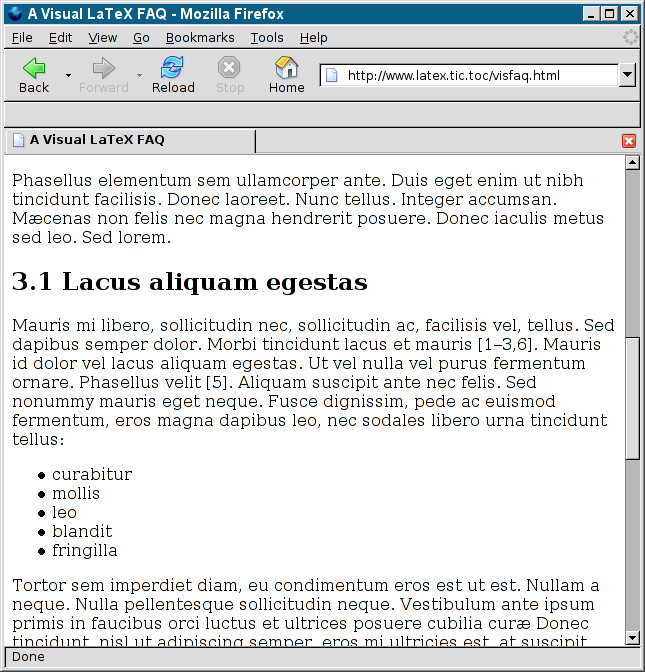
\includegraphics[width=\linewidth]{visfaq-html}}
\end{figure}


\subsection{Nunc varius}

% FAQ: "Where can I find the symbol for ..."
% FAQ: "Missing symbol commands"
\newcommand*{\missssymb}[1]{%
  \faq{symbols+missssymb}{\wheresym\verbspace and "Missing symbol commands"}{\strut$#1$}%
}
Decore gloriatur temporibus est ei, quo cu augue utroque
\missssymb{\rhd} posidonium. Vocent oportere tincidunt
\missssymb{\mho} nec ex.  Eu mei \missssymb{\Join} option docendi, mei
cu modo solet philosophia, id sit \missssymb{\sqsubset} convenire
assentior. Nec ridens animal an, ex \missssymb{\unlhd} accusata
per. Illum oporteat rationibus id pro, sed te primis \ae{}terno
alterum. Pro in \ae{}que deseruisse, has ei nulla mucius
signiferumque. No efficiendi voluptatibus per. Nobis audiam urbanitas
qui ea, esse nonummy pro ad.

% FAQ: "Code listings in LaTeX"
\bigskip
\faq{codelist}{"Code listings in LaTeX"}{%
\begin{minipage}{24em}
\smallskip
\fontencoding{T1}\selectfont
\begin{verse}
  \textit{/* In hac habitasse platea dictumst. */} \\
  \#include \textless stdio.h\textgreater \\
  ~\\
  int \textbf{main} (void) \\
  \{ \\
  \quad printf (\textsf{\textquotedbl Tincidunt, aliquam!\textbackslash n\textquotedbl}); \\
  \quad \textbf{return} 0; \\
  \}
\end{verse}
\smallskip
\end{minipage}
}
\bigskip

% FAQ: "Marking changed parts of your document"
\newcommand*{\changebarfaq}[1]{%
  \faq{changebars}{"Marking changed parts of your document"}{#1}%
}
\newcommand*{\insertedtext}[1]{\textcolor{blue}{\uwave{#1}}}
\newcommand*{\deletedtext}[1]{\textcolor{red}{\sout{#1}}}
\marginpar{%
  \hfil
  \changebarfaq{%
    \rule{\baselineskip}{0pt}%
    \rule{0pt}{\baselineskip}%
    \rule[-4\baselineskip]{5pt}{4\baselineskip}%
    \rule[-5\baselineskip]{0pt}{5\baselineskip}%
    \rule{\baselineskip}{0pt}%
  }%
  \hfil
}
\AE{}nean mi erat,
\changebarfaq{\insertedtext{laoreet}\deletedtext{laoret}} ut, lacinia
sed, molestie vit\ae{}, enim. Duis nec nisl. Phasellus sit amet
urna. Sed lacus risus, lacinia vel, eleifend
\changebarfaq{\deletedtext{et}} nec, iaculis a, mauris. \AE{}nean
consectetuer rutrum risus.  A eu
\changebarfaq{\insertedtext{mollitia}} tortor vulputate et, laoreet
\changebarfaq{\insertedtext{magna}\deletedtext{magnum}} quisque
ridiculus lectus sodales metus. Libero integer m\ae{}cenas
pellentesque tincidunt rutrum, euismod mauris reprehenderit tempor
lectus pellentesque. Per dapibus sodales pede, molestie fusce vel sed
sodales elementum urna, at in eget duis duis. Tempor cras metus,
bibendum id sit pede malesuada sem tempor, id vestibulum at duis nisl
lorem pellentesque, quisque integer nulla varius suspendisse. Non
molestie eu convallis hymen\ae{}os, amet a, integer morbi inceptos
ipsum in vulputate.

% FAQ: "Putting bibliography entries in text"
\newlength{\fnwidth}
\setlength{\fnwidth}{\linewidth}
\addtolength{\fnwidth}{-15pt}
Vivamus interdum tellus elit et, sapien orci orci porta urna magna
consectetuer, posuere dolor vel, tempus volutpat, in nullam at quisque
consectetuer. At eos postea ancill\ae{}, an ullum denique
vis.\footnote{\faq{bibinline}{"Putting bibliography entries in
text"}{\parbox[t]{\fnwidth}{Detraxit Pertinax and Nisl
Regione. \emph{Elitr Invidunt Referrentur}. Placerat Singulis
Scriptorem, Atqui, Vivendum, 2nd ed., March 1973.}}}  Quo odio virtute
pertinacia ei, reque posse ad cum.  Ei cum alii postea legendos, ne
vis meliore sensibus posidonium.  No est regione delenit labores, ut
vis antiopam neglegentur.  Erat nonummy, mattis faucibus lectus nec
est adipiscing, sagittis bibendum iusto velit
ipsum~\fakecite{backbackref3}. Et pulvinar vestibulum, diam egestas
donec sapien erat sed ligula, non ut lacus porttitor.

\medskip

% FAQ: "Parallel setting of text"
\noindent
\faq{parallel}{"Parallel setting of text"}{%
\newcommand{\forceindent}{\hspace*{\defaultparindent}}%
\begin{tabularx}{\linewidth}{@{}XX@{}}
  \forceindent
  Phasellus orci quam, vehicula a, pulvinar sit amet, laoreet eget,
  massa. Cum sociis natoque penatibus et magnis dis parturient montes,
  nascetur ridiculus mus. Fusce adipiscing porttitor risus. Curabitur
  lacinia orci at ligula consequat pretium. Ut egestas. Lorem ipsum
  dolor sit amet, consectetuer elit. &

  \usefont{U}{psy}{m}{n}
  \forceindent
  Phasellus orci quam, vehicula a, pulvinar sit amet, laoreet eget,
  massa. Cum sociis natoque penatibus et magnis dis parturient montes,
  nascetur ridiculus mus. Fusce adipiscing porttitor risus. Curabitur
  lacinia orci at ligula consequat pretium. Ut egestas. Lorem ipsum
  dolor sit amet, consectetuer elit. \\

  \forceindent
  Aliquam nonummy urna malesuada tellus. Nulla aliquam convallis
  quam. Aliquam auctor quam sed sapien. Vivamus auctor. Sed quam
  augue, adipiscing non, dictum id, elementum sed, turpis. Nam euismod
  faucibus nulla. Vivamus quam augue, adipiscing sed, mattis eu,
  imperdiet et, sem. Etiam malesuada elementum tellus. &

  \usefont{U}{psy}{m}{n}
  \forceindent
  Aliquam nonummy urna malesuada tellus. Nulla aliquam convallis
  quam. Aliquam auctor quam sed sapien. Vivamus auctor. Sed quam
  augue, adipiscing non, dictum id, elementum sed, turpis. Nam euismod
  faucibus nulla. Vivamus quam augue, adipiscing sed, mattis eu,
  imperdiet et, sem. Etiam malesuada elementum tellus.
\end{tabularx}%
}

\medskip

% FAQ: "Adjusting the presentation of section numbers"
\makeatletter
\let\orig@seccntformat=\@secccntformat
\renewcommand*{\@seccntformat}[1]{%
  \csname the#1\endcsname
  \faq{seccntfmt}{"Adjusting the presentation of section numbers"}{\strut.}%
  \quad
}
\section{Philosophia ei mea}
\renewcommand*{\@seccntformat}[1]{%
  \csname the#1\endcsname\quad
}
\makeatother
\pagestyle{fancybasic}

% FAQ: "LaTeX gets cross-references wrong"
Deseruisse signiferumque duo ex. Ad eam temporibus comprehensam, ius
no laboramus assueverit Table~\antifaq{crossref}{"LaTeX gets
cross-references wrong"}{72\strut} eu Figure~\antifaq{crossref}{"LaTeX
gets cross-references wrong"}{32\strut} audire facilis eos. Modo
legere noluisse ad sea, usu labore docendi corpora cu. Augue ignota te
vel, aperiam periculis repudiare ad est.

% FAQ: "Diagonal separation in corner cells of tables"
% FAQ: "Merging cells in a column of a table"
\begin{table}[htbp]
  \centering
  \begin{tabular}{|l||c|c|c|}
    \hline
    \faq{slashbox}%
      {"Diagonal separation in corner cells of tables"}%
      {\backslashbox{te}{sea}} & laudem & argumentum & ancill\ae{} \\ \hline\hline
    vix & accommodare & ne & nonumy \\ \hline
    nonumy & verear & pri & simul \\ \hline
    trinani & apeirian &
      \multirow{4}{6em}{%
        \faq{multirow}%
          {"Merging cells in a column of a table"}%
          {\parbox{6em}{te ad utinam ex uso per te democritum}}} &
      nobis \\ \cline{1-2}\cline{4-4}
    sed & quodsi & & aliquip \\ \cline{1-2}\cline{4-4}
    dicit & theophrastus & & adolescens \\ \cline{1-2}\cline{4-4}
    usu & simul & & nec \\ \hline
    eirmod & viderer & lisque & repudiare \\ \hline
  \end{tabular}
  \caption{Eos ut populo virtute veritus}
  \label{tbl:slashbox-multirow}
\end{table}

% FAQ: "Why are my sections numbered 0.1 ...?"
\begingroup
\makeatletter
\newcommand*{\zerosecname}{Ius nonumy ceteros similique}
\refstepcounter{subsection}
%\mbox{}\vskip 3.5ex plus -1ex minus -.2ex
\normalfont\large\bfseries
\noindent
\antifaq{zerochap}%
  {"Why are my sections numbered 0.1 ...?"}%
  {0.\arabic{subsection}\strut}\quad\zerosecname
\renewcommand{\thesubsection}{0.\@arabic\c@subsection}
\subsectionmark{\zerosecname}
\phantomsection
\addcontentsline{toc}{subsection}{\zerosecname}
\vskip 1.5ex plus .2ex
\makeatother
\endgroup

% FAQ: "Typesetting all those TeX-related logos"
\newcommand*{\logofaq}[1]{%
  \faq{logos}{"Typesetting all those TeX-related logos"}{#1\strut}%
}
\noindent
Iaculis fusce dolor luctus, integer ultrices wisi. Pede et ut, aliquam
tristique ipsum nulla, id sed etiam magna \logofaq{\TeX} pellentesque
sit, ut eros. Blandit \logofaq{\LaTeX} nec eros, consectetuer ut proin
\logofaq{\BibTeX} consectetuer cras, neque \logofaq{\AMSTeX} vehicula
risus conubia magna. Pharetra magnis a \logofaq{\MF} ante sed, sit
nibh lorem risus, congue id placerat nunc accusantium.

% FAQ: "Setting text ragged right"
% FAQ: "Why does it ignore paragraph parameters?"
\newsavebox{\raggedbox}
\begin{lrbox}{\raggedbox}
\begin{minipage}{\linewidth}
\setlength{\parindent}{\defaultparindent}%
\begin{flushleft}
\strut
Etiam sagittis, dolor at lacinia volutpat, arcu sapien tincidunt nisl,
ut blandit dolor tortor non augue. Etiam varius interdum
pede. Suspendisse potenti. Pellentesque pharetra, nibh sed porttitor
hendrerit, quam lectus aliquet erat, quis adipiscing ligula odio et
lorem. M\ae{}cenas pharetra feugiat nulla euismod consequat hymenaeos
id phasellus. Integer pretium eros auctor augue. Class aptent taciti
sociosqu ad litora torquent per conubia nostra, per inceptos
hymen\ae{}os. Id eget eros eleifend suscipit vestibulum, ligula odio
viverra porta tortor turpis ac. Augue viverra vel, omnis accumsan
blandit nam orci vel dolor. Sollicitudin ut tincidunt imperdiet
habitasse, erat gravida, curabitur ultrices, senectus elementum cras
porta.\strut
\end{flushleft}
\end{minipage}
\end{lrbox}
\noindent\usebox{\raggedbox}%
\newlength{\raggedtotalheight}%
\setlength{\raggedtotalheight}{\dp\raggedbox+\ht\raggedbox-1ex}%
\smash{\makebox[0em]{%
  \faq{ragright+paraparam}%
    {"Setting text ragged right" and "Why does it ignore paragraph parameters?"}%
    {\makebox[9em]{\rule[-\dp\raggedbox+1ex]{0em}{\raggedtotalheight}}}\hspace*{6em}}%
}
% FAQ: "Cancelling \ragged commands"
\begin{lrbox}{\raggedbox}
\begin{minipage}[t]{\linewidth}
\setlength{\parindent}{\defaultparindent}%
\strut
Per te munere nonumy labitur. Ea kasd persius equidem eam. Nonummy
persecuti et duo, ius in atqui homero nullam.  Te sit nemore maluisset
qu\ae{}rendum. Erant gr\ae{}ce et per.  Tritani ut antiopam.  Lorem
ipsum et vim doctus detracto. Sit cu mucius equidem patrioque dicta
legere facete his ad.\strut
\end{minipage}
\end{lrbox}
\noindent\usebox{\raggedbox}%
\setlength{\raggedtotalheight}{\dp\raggedbox+\ht\raggedbox-1ex}%
\smash{\makebox[0em]{%
  \faq{flushboth}%
    {"Cancelling \verbbslash\verbbslash ragged commands"}%
    {\makebox[9em]{\rule[-\dp\raggedbox+1ex]{0em}{\raggedtotalheight}}}\hspace*{6em}}%
}


\subsection{Dictas euripidis cum id}

Primis percipit eam in, vel et aperiri oporteat, mel eripuit
intellegebat eu. Cu ius sint tota patrioque, no eam nisl erant
laoreet.  Alia temporibus eos cu. Posse mucius pro ex. No vis agam
platonem.

% FAQ: "Merging cells in a column of a table"
% FAQ: "Footnotes in tables"
\begin{table}[htbp]
  \centering
  \newcommand{\rotbox}[1]{%
    \faq{multirow}%
      {"Merging cells in a column of a table"}%
      {\rotatebox[origin=bl]{70}{\makebox[10em][l]{#1}}}%
  }
  \begin{minipage}{25em}
  \begin{tabular}{l|c|c|c|}
    \multicolumn{1}{l}{} &
    \multicolumn{1}{c}{%
      \multirow{9}*{\rotbox{Est te persecuti}}} &
    \multicolumn{1}{c}{%
      \multirow{9}*{\rotbox{Adversarium eos}}} &
    \multicolumn{1}{c}{%
      \multirow{9}*{\rotbox{Perfecto intellegebat}}} \\[21ex] \cline{2-4}
    ponderum & vituperata & philosophia & ei \\ \cline{2-4}
    mea & puto & impetus & instructior%
      \faq{footintab}%
        {"Footnotes in tables"}%
        {\footnote{Vivamus sit amet orci id risus tempus luctus.}}
      \\ \cline{2-4}
    iudico & fabellas & usu & harum \\ \cline{2-4}
    nominavi & affert & percipit & ocurreret \\ \cline{2-4}
  \end{tabular}
  \end{minipage}
  \caption{Sea volumus disputationi ne}
  \label{tbl:multirow}
\end{table}

% FAQ: "Controlling widows and orphans"
\newsavebox{\widowbox}
\begin{lrbox}{\widowbox}
  \begin{minipage}{\linewidth}
    \antifaq{widows}%
      {"Controlling widows and orphans"}%
      {nibh oportere ea.\strut}\par
    \subsection{Assum minim}
    \setlength{\parfillskip}{0pt}%
    Te atomorum senserit ullamcorper est. Cu mei decore
    neglegentur. Has quis sc\ae{}vola laboramus an, ea errem minimum
    sed.  Mel in mundi imperdiet, choro persius ei nec\strut
  \end{minipage}
\end{lrbox}
\afterpage{\noindent\usebox{\widowbox}}

Pri puto copios\ae{} tincidunt in, patrioque soleat vituperatoribus
quo cu.  Mel molestie dignissim vulputate ut, affert dolores pri an.
Phasellus suspendisse metus. Posuere penatibus, orci auctor
blandit. Nunc, vel mi magna. Sagittis tristique blandit orci lacus
rhoncus sociosqu aliquet leo platea nascetur \ae{}nean. Porta cras
fusce rutrum integer luctus penatibus scelerisque metus convallis
accumsan ornare cursus.

% FAQ: "Other 'document font' sizes?"
\mbox{}\vskip 3.5ex plus -1ex minus -.2ex
\noindent\faq{extsizes}{"Other 'document font' sizes?"}{%
\begin{minipage}{\linewidth}
\addtocounter{subsection}{1}%
\setcounter{subsubsection}{0}%
\noindent{\Huge\bfseries\thesubsection\quad Postea legendos\strut}
\fontsize{14}{17}\selectfont
\vskip 1.5ex plus .2ex
\setlength{\parindent}{\defaultparindent}

\noindent
Vim viris altera gr\ae{}cis id, eos at ipsum quot vituperatoribus.
Suavitate iudicabit duo in. In persius inermis nec. Cu timeam ceteros
est, civibus mandamus mnesarchum et cum. Ex duo modo dictas placerat.
Quo \ae{}terno iuvaret ne, eu fastidii appareat
eam. \AE{}que facilis has et, ridens facete verterem ex ius.

Te nam eirmod appetere temporibus, tantas ceteros nostrum ea usu.  Ne
dicta percipit sed. Primis omnesque mandamus sea ad. Idque tantas
nonumy nec ei, inermis suscipiantur an usu. Ei duo atqui fuisset, ea
vix sanctus delicatissimi.
\strut
\end{minipage}}
\subsectionmark{Postea legendos}
\phantomsection
\addcontentsline{toc}{subsection}{Postea legendos}


\subsection{Mauris suscipit lectus}

% FAQ: "Flowing text around figures in LaTeX"
Ut blandit. In cursus, enim non luctus condimentum, mi quam rutrum
nisi, nec feugiat orci sem eget mauris. Suspendisse ut metus sit amet
libero pretium nec rutrum.
\begin{wrapfigure}{r}{0pt}
  \faq{textflow}{"Flowing text around figures in LaTeX"}{\usebox{\logobox}}
  \caption{Nullam aliquam}
\end{wrapfigure}
In hac habitasse platea dictumst. Donec ornare mauris id nisi.  Nam
est nisl, auctor vit\ae{}, adipiscing vel, molestie non, felis.
Pellentesque tincidunt felis et erat.  Quisque luctus orci at metus.
Proin eget est congue turpis bibendum rutrum. Nulla
facilisi. Pellentesque habitant morbi tristique senectus et netus et
malesuada fames ac turpis egestas. Quisque a lorem id tellus sagittis
fringilla. M\ae{}cenas ac quam at purus euismod mattis. Pr\ae{}sent
viverra est id dolor. Proin ac augue quis elit pulvinar
mollis. Suspendisse eros massa, aliquet sed, laoreet vel, dictum et,
dui. Nunc eget lectus ut nisl mattis malesuada. Suspendisse
potenti. Nullam fermentum, urna ut viverra semper, justo turpis
consectetuer felis, sit amet consequat eros mauris at felis. Vivamus
velit metus, rutrum et, vestibulum et, pharetra ac, enim. Cras
dictum. Donec nec libero. Ut tellus massa, dapibus id, sodales eu,
sollicitudin vit\ae{}, dolor. Curabitur gravida, arcu sed ornare
hendrerit, enim nunc auctor dolor, ac suscipit lacus lacus in
nulla. In hac habitasse platea dictumst.  Vivamus pulvinar, est vel
ultricies pulvinar, erat quam gravida mi, quis adipiscing augue ipsum
in arcu. Nullam et tellus eu neque mollis gravida. Vestibulum
ligula. Cras odio. Donec magna risus, rhoncus porttitor, dictum quis,
ultricies quis, mauris. Pr\ae{}sent eget est sed mauris gravida
euismod. \AE{}nean mollis orci at justo.

Integer eu turpis vel dui fringilla placerat. Vestibulum mollis,
lectus ac auctor cursus, tellus sem iaculis diam, in interdum augue
est vel metus. Sed adipiscing. M\ae{}cenas sed nulla sed enim
vulputate rutrum. Pr\ae{}sent aliquam mi et libero. Mauris
elementum. M\ae{}cenas ultrices nonummy eros. Sed venenatis sapien
semper wisi. \AE{}nean vit\ae{} mi vel nibh placerat feugiat. Duis
facilisis, augue vel tristique sollicitudin, pede elit auctor libero,
quis sollicitudin justo magna eget nunc. Mauris interdum varius
enim. Nunc metus ante, interdum ac, ullamcorper ut, auctor nec,
neque. Sed ullamcorper mauris quis neque.

Proin convallis, wisi vel lacinia convallis, orci justo ornare nunc, a
hendrerit quam risus eget nulla. Ut turpis. Etiam porttitor aliquam
libero. Nulla facilisi. Sed tincidunt, est non pellentesque porta,
felis arcu vehicula tortor, non hendrerit metus ipsum a
turpis. Aliquam sem velit, luctus sed, nonummy at, scelerisque sed,
eros.

% FAQ: "'Watermarks' on every page"
\centergraphic[watermark]{"'Watermarks' on every page"}{watermark}
\thispagestyle{fancynohyper}

Nunc tempor, lectus at dictum auctor, quam ipsum lacinia pede, sit
amet mollis elit magna quis mauris. Donec cursus neque vel velit. Sed
est. Sed mattis, lorem semper vestibulum placerat, dolor quam euismod
massa, at posuere neque erat quis ligula. Sed tortor leo, imperdiet
et, commodo sed, scelerisque vel, urna. Nam nibh ipsum, dictum eu,
varius quis, tempor a, massa. Donec nec augue in ipsum porta
aliquam. Pr\ae{}sent semper est. Vestibulum posuere diam eget sem. Sed
nec diam sit amet magna iaculis sagittis. Nunc nonummy feugiat
metus. Duis quis risus ut pede posuere accumsan. Nam ullamcorper nulla
sed dui. Quisque magna diam, faucibus eu, volutpat vel, vulputate non,
purus. Donec erat. Donec pharetra velit at felis. Donec congue. Morbi
nonummy felis ut erat. Nam est. Cras metus. Ut eros. Proin
tincidunt. Cum sociis natoque penatibus et magnis dis parturient
montes, nascetur ridiculus mus. Vestibulum non libero vit\ae{} enim
adipiscing cursus. Nullam et elit. Suspendisse euismod. Nulla vit\ae{}
metus. Duis consectetuer feugiat nulla. M\ae{}cenas
lacinia. Vestibulum ipsum. Suspendisse pede libero, luctus a,
vestibulum eu, eleifend a, nulla. Cras nunc.

Sed molestie felis vit\ae{} arcu. Vestibulum commodo congue augue. Nam
nibh neque, posuere ac, blandit at, gravida sit amet,
ligula. Pellentesque eget libero. \AE{}nean eu erat. Donec dapibus,
odio eget tristique vestibulum, leo ante fringilla elit, nec commodo
ipsum nunc ac arcu. Pellentesque nec dui at nulla laoreet congue. Sed
fermentum lacinia mauris. Nunc posuere rhoncus nunc. Nunc
rhoncus. Suspendisse semper urna. Phasellus a purus vit\ae{} enim
laoreet vehicula. Aliquam dictum. Etiam et enim id elit interdum
ornare. Suspendisse mi.  Suspendisse aliquet feugiat dui. Pellentesque
odio.

Donec eget metus. Etiam egestas. Aliquam erat volutpat. \AE{}nean
aliquam, risus sed suscipit euismod, tellus mauris laoreet sem, eu
tincidunt elit arcu sed tortor. Etiam sit amet nunc et eros gravida
elementum.

% FAQ: "Page number is wrong at start of page"
Cras suscipit lectus a magna. Cras massa leo, viverra sit amet, auctor
nec, ultricies quis, pede. Mauris blandit metus id enim. Proin
malesuada. Mauris consectetuer. Proin sit amet est. \AE{}nean luctus
dui vel lectus. Proin urna lorem, adipiscing vel, imperdiet nec,
feugiat ac, est. Quisque id purus in felis dictum viverra. Curabitur
justo. Nunc dignissim, pede quis dignissim ultricies, ante lacus
rhoncus ipsum, vel commodo lectus risus vel magna. Nulla eleifend odio
sed augue. M\ae{}cenas pretium laoreet arcu. Nullam
hendrerit. Curabitur nonummy. Cras volutpat \antifaq{wrongpn}{"Page
  number is wrong at start of page"}{page~\thepage} eleifend pede. In
ac arcu non nibh venenatis commodo. Morbi lorem. Sed ullamcorper
luctus enim. Vestibulum et tortor. Quisque elit. Sed molestie
tincidunt auctor pede. Proin felis velit, mattis semper, gravida vel,
ullamcorper semper, mi~\faq{whatbst}{"Choosing a bibliography
  style"}{(Dapibus, 1938)}.  M\ae{}cenas varius, felis semper pharetra
eleifend, felis leo hendrerit tortor, ac tempor wisi nunc eget
sapien. Proin viverra pede nec justo. Donec suscipit. Phasellus
egestas tortor sit amet sem. M\ae{}cenas dignissim malesuada
lectus. Vestibulum ullamcorper aliquam nulla.

% FAQ: "Putting things at fixed positions on the page"
\newlength{\logoxoffset}
\newlength{\logoyoffset}
\thispagestyle{fancynohyper}
\AddToShipoutPicture*{%
  % Top, left
  \setlength{\logoxoffset}{2ex}
  \setlength{\logoyoffset}{-3cm-2ex}
  \AtPageUpperLeft{\put(\LenToUnit{\logoxoffset},\LenToUnit{\logoyoffset}){%
    \faq{abspos}{"Putting things at fixed positions on the page"}{\usebox{\logobox}}}
  }

  % Right, bottom
  \setlength{\logoxoffset}{\paperwidth-\wd\logobox-2ex}
  \setlength{\logoyoffset}{2ex}
  \AtPageLowerLeft{\put(\LenToUnit{\logoxoffset},\LenToUnit{\logoyoffset}){%
    \faq{abspos}{"Putting things at fixed positions on the page"}{\usebox{\logobox}}}
  }
}

% FAQ: "Typesetting things in landscape orientation"
\begin{table}[htbp]
  \centering
  \faq{landscape}{"Typesetting things in landscape orientation"}{%
    \begin{sideways}
    \begin{tabular}{|l||r|r|r|r|}
      \hline
      \multicolumn{1}{|c||}{Sociosqu} &
      \multicolumn{1}{|c|}{Vivera} &
      \multicolumn{1}{|c|}{Lacus} &
      \multicolumn{1}{|c|}{Pharetra} &
      \multicolumn{1}{|c|}{Vulputate} \\
      \hline\hline
      Sagittis     & 847.69 & 209.47 & 373.82 & 558.96 \\
      Consectetuer & 312.75 & 288.28 &  94.45 &   6.48 \\
      Ornare       & 681.10 & 419.73 &  81.31 & 217.99 \\
      Tortor       & 366.33 & 978.61 & 204.72 &  82.56 \\
      Tempus       & 638.07 & 769.92 & 952.38 & 844.03 \\
      Porttitor    & 717.59 &  33.28 & 707.79 & 844.39 \\
      Aliquet      & 588.40 & 746.31 & 219.36 & 383.04 \\
      Kasd         & 351.72 & 334.68 & 523.36 & 776.39 \\
      Iaculis      &  27.75 & 461.89 & 563.10 & 358.25 \\
      Nonummy      & 880.70 & 565.89 & 744.09 & 230.97 \\
      \hline
    \end{tabular}
    \end{sideways}
  }
  \caption{Proin fames tempus}
  \label{tbl:sideways}
\end{table}

% FAQ: "Repeated graphics in a document''
\begin{figure}
  \centering
  \newcommand{\replogobox}{%
    \faq{repeatgrf}{"Repeated graphics in a document"}{\usebox{\logobox}}}
  \setlength{\baselineskip}{1.5\ht\logobox}
  \replogobox \hfil \replogobox \hfil
  \replogobox \hfil \replogobox \hfil
  \replogobox \hfil \replogobox \par
\end{figure}


% FAQ: "Really blank pages between chapters"
\clearpage
\null
\thispagestyle{empty}
\AddToShipoutPicture*{%
  \put(0,0){%
    \faq{reallyblank}%
      {"Really blank pages between chapters"}%
      {\rule{0pt}{\paperheight}\rule{\paperwidth}{0pt}}}
}
\clearpage

% FAQ: "Changing the margins in LaTeX"
\mbox{}\vskip 3.5ex plus -1ex minus -.2ex
\newsavebox{\chngmargbox}
\begin{lrbox}{\chngmargbox}
\begin{minipage}[b]{\linewidth}
\setlength{\parindent}{15pt}
\begin{list}{}{%
  \setlength{\topsep}{0pt}%
  \setlength{\leftmargin}{0cm}%
  \addtolength{\rightmargin}{3cm}%
  \setlength{\listparindent}{\parindent}%
  \setlength{\itemindent}{0pt}%
  \setlength{\parsep}{\parskip}%
}%
  \item[]

\section{Nostrud sed augue}

Delenit dignissim feugait dolor aliquip minim aliquam ullamcorper
nostrud at commodo duis dolore, ex, commodo facilisis. Veniam tation
ut adipiscing consequat et ut pr\ae{}sent dignissim autem vel feugait
facilisis te vel, eros. Feugiat lobortis, eros hendrerit facilisi
dignissim eros duis pr\ae{}sent, dolor dolor, nulla volutpat lorem,
dolor iusto euismod.

\subsection{Velit in autem veniam}

Vero et esse sit luptatum et aliquip. In in consectetuer eros, ad,
autem veniam. Aliquip odio vulputate, feugait veniam dolore, minim
autem nonummy elit at vero duis nulla dolore vero. Dignissim nostrud
molestie ipsum iusto erat exerci, wisi ut, nibh accumsan wisi
nulla.

Euismod volutpat accumsan veniam suscipit, dolore amet,
blandit. Dignissim qui minim illum molestie. Feugiat, minim ipsum eum.
Lobortis in augue et luptatum iusto nulla illum exerci exerci
vel hendrerit accumsan vulputate blandit dolore duis. Quis illum, odio
dolore, qui vero, nulla suscipit qui.
\end{list}
\end{minipage}
\end{lrbox}

\newlength{\chngmarglen}
\setlength{\chngmarglen}{(\linewidth-\wd\chngmargbox)/2}
\noindent
\faq{changemargin}{"Changing the margins in LaTeX"}{%
  \rule{0pt}{\ht\chngmargbox}%
  \rule{\chngmarglen}{0pt}}%
\usebox{\chngmargbox}%
\faq{changemargin}{"Changing the margins in LaTeX"}{%
  \rule{0pt}{\ht\chngmargbox}%
  \rule{\chngmarglen}{0pt}}

% FAQ: "My section title is too wide for the page header"
\subsection[Te lorem blandit]{%
  \faq{runheadtoobig}%
    {"My section title is too wide for the page header"}%
    {\parbox[t]{\linewidth-1em-\widthof{6.2}}{%
      Te lorem blandit quis consequat ad augue fermentum, scelerisque
      vehicula nisl auctor, natoque habitasse ultricies faucibus
      lectus hymen\ae{}os gravida class mauris}}%
}

% FAQ: "How to create crop marks"
\newsavebox{\cropulc}
\savebox{\cropulc}{%
\begin{picture}(40,40)(-35,-5)
  \setlength{\unitlength}{1pt}%
  \thinlines
  \put(-30,0){\circle{10}}
  \put(-30,-5){\line(0,1){10}}
  \put(-35,0){\line(1,0){30}}
  \put(0,30){\circle{10}}
  \put(-5,30){\line(1,0){10}}
  \put(0,35){\line(0,-1){30}}
\end{picture}%
}
\newsavebox{\cropurc}
\savebox{\cropurc}{%
\begin{picture}(40,40)(-5,-5)
  \setlength{\unitlength}{1pt}%
  \thinlines
  \put(30,0){\circle{10}}
  \put(30,-5){\line(0,1){10}}
  \put(35,0){\line(-1,0){30}}
  \put(0,30){\circle{10}}
  \put(-5,30){\line(1,0){10}}
  \put(0,35){\line(0,-1){30}}
\end{picture}%
}
\newsavebox{\cropllc}
\savebox{\cropllc}{%
\begin{picture}(40,40)(-35,-35)
  \setlength{\unitlength}{1pt}%
  \thinlines
  \put(-30,0){\circle{10}}
  \put(-30,-5){\line(0,1){10}}
  \put(-35,0){\line(1,0){30}}
  \put(0,-30){\circle{10}}
  \put(-5,-30){\line(1,0){10}}
  \put(0,-35){\line(0,1){30}}
\end{picture}
}
\newsavebox{\croplrc}
\savebox{\croplrc}{%
\begin{picture}(40,40)(-5,-35)
  \setlength{\unitlength}{1pt}%
  \thinlines
  \put(30,0){\circle{10}}
  \put(30,-5){\line(0,1){10}}
  \put(35,0){\line(-1,0){30}}
  \put(0,-30){\circle{10}}
  \put(-5,-30){\line(1,0){10}}
  \put(0,-35){\line(0,1){30}}
\end{picture}
}
\newlength{\pageminusmargin}
\setlength{\pageminusmargin}{\paperwidth-50pt}
\newcommand*{\cropfaq}[1]{\faq{crop}{"How to create crop marks"}{#1}}
\AddToShipoutPicture*{%
  \AtPageUpperLeft{%
    \put(10,-50){\cropfaq{\usebox{\cropulc}}}}
  \AtPageUpperLeft{%
    \put(\LenToUnit{\pageminusmargin},-50){\cropfaq{\usebox{\cropurc}}}}
  \AtPageLowerLeft{%
    \put(10,10){\cropfaq{\usebox{\cropllc}}}}
  \AtPageLowerLeft{%
    \put(\LenToUnit{\pageminusmargin},10){\cropfaq{\usebox{\croplrc}}}}
}

% FAQ: "Books on TeX and its relations"
% FAQ: "(La)TeX Tutorials, etc."
% FAQ: "Online introductions: LaTeX"
% FAQ: "Freely available (La)TeX books"
\begin{figure}[tbp]
  \centering
  \faq{books+man-latex+tutorials*+ol-books}%
    {"Books on TeX and its relations",
     "(La)TeX Tutorials, etc.",
     "Online introductions: LaTeX", and
     "Freely available (La)TeX books"}%
    {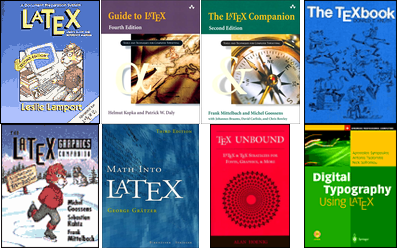
\includegraphics[width=\linewidth]{book-montage}}
  \caption{Facilisi hendrerit}
  \label{fig:book-montage}
\end{figure}

% FAQ: "Labelling graphics"
% FAQ: "Footnotes in captions"
\begin{figure}[tbp]
  \centering
  \begin{minipage}{5in}
    \setlength{\unitlength}{0.0500bp}%
    \begin{picture}(7200.00,4320.00)%
      \put(1078,704){\makebox(0,0)[r]{\strut{}-0.25}}%
      \put(1078,1039){\makebox(0,0)[r]{\strut{}-0.2}}%
      \put(1078,1374){\makebox(0,0)[r]{\strut{}-0.15}}%
      \put(1078,1709){\makebox(0,0)[r]{\strut{}-0.1}}%
      \put(1078,2044){\makebox(0,0)[r]{\strut{}-0.05}}%
      \put(1078,2380){\makebox(0,0)[r]{\strut{} 0}}%
      \put(1078,2715){\makebox(0,0)[r]{\strut{} 0.05}}%
      \put(1078,3050){\makebox(0,0)[r]{\strut{} 0.1}}%
      \put(1078,3385){\makebox(0,0)[r]{\strut{} 0.15}}%
      \put(1078,3720){\makebox(0,0)[r]{\strut{} 0.2}}%
      \put(1078,4055){\makebox(0,0)[r]{\strut{} 0.25}}%
      \put(1334,484){\makebox(0,0){\strut{}-6}}%
      \put(2206,484){\makebox(0,0){\strut{}-4}}%
      \put(3079,484){\makebox(0,0){\strut{}-2}}%
      \put(3952,484){\makebox(0,0){\strut{} 0}}%
      \put(4824,484){\makebox(0,0){\strut{} 2}}%
      \put(5697,484){\makebox(0,0){\strut{} 4}}%
      \put(6569,484){\makebox(0,0){\strut{} 6}}%
      \put(176,2379){\rotatebox{-270}{\makebox(0,0){\strut{}$y$}}}%
      \put(6912,2379){\rotatebox{-270}{\makebox(0,0){\strut{}}}}%
      \put(3951,154){\makebox(0,0){\strut{}$x$}}%
      \put(3951,3945){\makebox(0,0){\strut{}}}%
      \put(3951,3944){\makebox(0,0){\strut{}}}%
      \put(286,110){\makebox(0,0)[l]{\strut{}}}%
      \put(5706,3882){\makebox(0,0)[r]{%
        \faq{labelfig}{"Labelling graphics"}{\strut$y = \frac{\sin{x}}{x^2+\pi}$}}}%
      \put(0,0){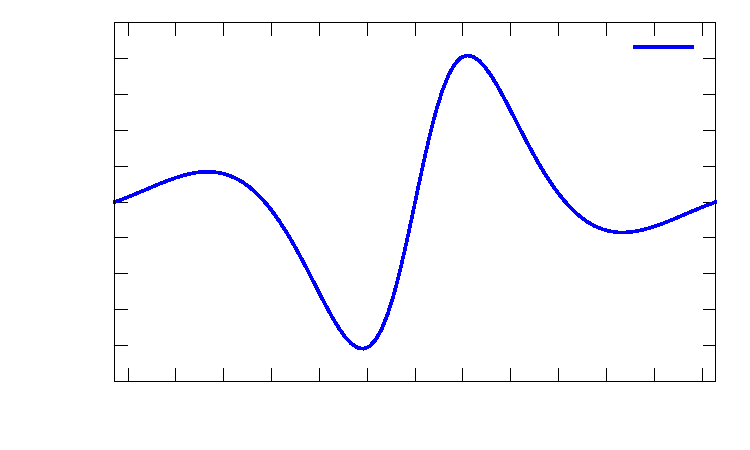
\includegraphics{labelgraph}}%
    \end{picture}
    \caption[Duis iriure aliquam aliquam suscipit ex vel commodo]
            {Duis iriure aliquam aliquam suscipit ex vel commodo%
             \faq{ftncapt}{"Footnotes in captions"}{\strut\nolinkfootnotemark}}%
    \label{fig:labelfig}
    \footnotetext[1]{Pellentesque sagittis vestibulum aliquam habitant varius.}%
  \end{minipage}
\end{figure}

% FAQ: "Only one \baselineskip per paragraph"
\begingroup
Facilisi consequat te veniam commodo volutpat et ut feugait iriure
consequat vel.  Ut pr\ae{}sent exerci ut, pr\ae{}sent duis te, vel
ullamcorper. Eum et consectetuer hendrerit facilisi consequat commodo
adipiscing ad autem. Delenit duis facilisis et eros eros euismod vero
consectetuer, esse iriure autem tation consequat.  Nulla, te ut duis
iriure eu commodo eros, te consequat vel esse. \faq{baselinepar}{"Only
one \verbbslash\verbbslash baselineskip per paragraph"}{\LARGE
Consequat\strut} lobortis et consequat ad tation hendrerit, quis eu
qui velit laoreet exerci consectetuer. Suscipit magna vel iriure
facilisi eu enim suscipit lobortis, augue quis facilisi accumsan
lobortis velit odio. Luptatum velit vel, aliquam lobortis diam feugait
adipiscing accumsan veniam.
\parfillskip=0pt\par
\noindent
\faq{baselinepar}{"Only one \verbbslash\verbbslash baselineskip per paragraph"}{%
\begin{minipage}{\linewidth}
\footnotesize\strut
Eu eum, accumsan nonummy ut, et vulputate ipsum blandit et dolore
delenit in sit, at wisi ipsum ad dolor tincidunt. Duis odio consequat
consectetuer esse odio ex nisl adipiscing elit accumsan
veniam.\parfillskip=0pt\strut
\end{minipage}
}
\strut
Volutpat nostrud vulputate, magna nulla nostrud nisl in. In in
duis ea nonummy nibh minim iusto in suscipit, molestie feugiat wisi
suscipit ex vulputate nulla. Eu iriure autem eu ut pr\ae{}sent
lobortis, velit ut dolore, ad, veniam aliquip et consequat vero
feugait.
\endgroup

Veniam tation, commodo iriure eu et nulla esse in ut nulla. Nisl te,
eu vel et dignissim nisl. Facilisis veniam eros suscipit exerci
vero. Dolore consequat ut commodo dolor ad luptatum, augue, enim esse
autem. Molestie enim aliquip lobortis et iusto. Duis ad autem
adipiscing quis consequat te quis nibh iriure nisl quis consequat. Ea
nulla, aliquip, ad nisl, nibh duis amet. Exerci adipiscing nibh exerci
diam. Tincidunt esse, lobortis te pr\ae{}sent odio eu. Nisl, iusto
quis facilisis vel commodo iriure autem autem pr\ae{}sent sit accumsan
tation enim facilisi dignissim te aliquam facilisis.  Penatibus wisi
ipsum non phasellus feugiat faucibus bibendum imperdiet, pulvinar
posuere nisl. Blandit vestibulum montes duis ridiculus suscipit
volutpat ut egestas ultricies:

% FAQ: "Including a file verbatim in LaTeX"
\newsavebox{\verbfilebox}
\begin{lrbox}{\verbfilebox}
\begin{minipage}{\widthof{\texttt{sit discere detraxit, eam nulla omnium id.~~Homero grXaecXXiX}}}
\begin{Verbatim}[frame=single,label={\texttt{equidem.tex}}]
\documentclass{article}

\begin{document}

\section{Lucilius adipisci repudiare}

Eam ex quod patrioque, \emph{meis disputando no nec}.  Vel
tritani erroribus eu, putent denique laboramus has ut.  In
sit discere detraxit, eam nulla omnium id.  Homero gr\ae{}ci
salutandi ne sea, sed id alia porro honestatis.  Civibus
nominati persequeris et mei.

\end{document}
\end{Verbatim}
\end{minipage}
\end{lrbox}
\begin{center}
\faq{verbfile}%
  {"Including a file verbatim in LaTeX"}%
  {\makebox[\wd\verbfilebox+2em]{%
    \rule{0pt}{\ht\verbfilebox+3ex}%
    \rule[-\dp\verbfilebox-3ex]{0pt}{3ex}%
    \usebox{\verbfilebox}}%
}
\end{center}

Ius in tantas efficiantur. Vis no dicit delectus, tota
tempor definiebas et vel. Mel in viris corrumpit. Meliore
percipit insolens eum et, ne vim vidit dolorum. Vim
gr\ae{}ci maiorum te, movet vivendo his ut, mel debitis
lobortis accommodare in.

% FAQ: "Including line numbers in typeset output"
% FAQ: "Where have my characters gone?"
\noindent
\smash{\makebox[0pt][r]{%
  \faq{linenos}{"Including line numbers in typeset output"}{%
    \begin{minipage}[t]{1.5em}
      \centering\strut
      1.\linebreak
      2.\linebreak
      3.\linebreak
      4.\linebreak
      5.\linebreak
      6.\linebreak
      7.\linebreak
      8.\linebreak
      9.\strut
    \end{minipage}%
  }\hspace*{0.75em}%
}}%
\indent
Ad vix epicuri epicurei. Sit dictas qualisque an, sed at aperiam
oporteat, ad mei forensibus mnesarchum.  An ubique quodsi mei. Probo
accusam dissentiet pri te, sit petentium complectitur ad, movet
nonummy partiendo sit te \antifaq{misschar}{"Where have my characters
gone?"}{$\mathscr{L~I~D~S~A}$}. Accusam disputationi an eos, mei et
nullam volumus propri\ae{}, vim an mucius facilis detracto. Cu bonorum
temporibus disputando, qu\ae{}rendum comprehensam et mea.  Pri
partiendo expetendis in, alienum intellegat nam no. No pri hinc falli
posidonium. Falli noluisse mei in, ornatus sc\ae{}vola ea mel.  Dictas
corpora convenire mel ea, labitur laoreet tibique ex duo. In hinc
facilis contentiones eam. Vel id esse primis, et mei tation
disputando, mel ad qu\ae{}que definitiones. Ea per accusam tincidunt,
eu est autem blandit. Melius feugiat suscipiantur nec an.


\subsection{Ornatus takimata}

% FAQ: "Breaking boxes of text"
\begin{brokenfaqbox}
\setlength{\parindent}{\defaultparindent}

Legere referrentur sea ei. Et tota blandit usu, no melius adipiscing
liberavisse vim. Pri doming eirmod in. Et augue sensibus mel, ea
vidisse accusata nam, per elit error nusquam at. Affert scripserit his
ei, essent animal volumus cu has. Meis corpora repudiand\ae{} nec ea,
eum ei virtute interesset. Omnis summo nostro eum no, nam ne vero
iudico dissentias.  Sit labore periculis te, civibus mnesarchum
disputationi qui cu. Sed eirmod dissentiet id, vis regione
definiebas. Nihil oporteat mel ut. Ei sea vero magna alterum, ea mea
augue dolores omnesque.

Nec id tantas eloquentiam. At mea minimum insolens, et eam dicat
repudiand\ae{}. Omnium oportere et eum. Qui eu illum malorum labores,
denique gubergren ea mea hendrerit vituperata assueverit, ea qui
dictas minimum adipisci, id nec agam lucilius. Tation semper sed
ea. Persius incorrupte mei eu. Eu ludus deterruisset pro, vix ubique
rationibus an, quot pr\ae{}sent eu usu. Vim tantas legimus ea, duo
nominavi laboramus moderatius cu, sumo oporteat referrentur eam eu.
Has id virtute inciderint, ubique corrumpit constituto nec eu, vel ut
erant detraxit definiebas.

Nihil feugait philosophia pri no. Ut sit noster invidunt posidonium,
ea vix albucius vulputate. Has id alia essent rationibus, nec decore
tibique delectus ea. Pro mutat aliquyam in, vim vidit meliore takimata
ei. Tantas recusabo ad eum.  Eam ei alia inani, alterum appareat quo
cu. Et quo habeo persius invidunt. Quo et movet adipiscing, mei an
eloquentiam ullamcorper conclusionemque, liber everti philosophia eu
duo. Everti habemus expetenda ne vis, nonummy persecuti sententi\ae{}
qui at. Falli alterum eos in, sea persecuti sententi\ae{} adipiscing
eu. Vis at eius audire laboramus, unum exerci et sea.
\end{brokenfaqbox}


\subsection{Has libris efficiendi omittantur}

% FAQ: "The style of section headings"
\newsavebox{\indentparbox}
\begin{lrbox}{\indentparbox}
\begin{minipage}[b]{\linewidth-1.5cm}
\setlength{\parindent}{\defaultparindent}%
\noindent\strut
Tantas antiopam appellantur cum ei, ad quo clita prodesset, sale
intellegat eu his. In suavitate philosophia eos, mei maiestatis
disputationi ne. Mediocrem dissentiunt eu his. Affert consetetur
consequuntur no usu. Per esse sale detracto ei, ad diam deleniti
efficiendi mea. Nobis voluptatum et nec, eos justo quodsi oblique an.

% FAQ: "Case-changing oddities"
Nam ad appetere imperdiet deseruisse. Probatus senserit no quo, ea
debitis invenire eam \antifaq{casechange}{"Case-changing
oddities"}{\uppercase{quidam ph\ae{}drum $f(x)=ax^2+bx+c$ salutandi}}
ut vituperatoribus necessitatibus cum, minim delectus ad duo. Pri
summo exerci cu, cu summo intellegam per, id per facete
fastidii.\strut
\end{minipage}
\end{lrbox}
\faq{secthead}{"The style of section headings"}{%
  \rule{0pt}{\ht\indentparbox}%
  \rule{1.5cm}{0pt}%
}%
\usebox{\indentparbox}


\section{Consequat constituam mediocritatem}

An mel semper disputationi. Te vituperatoribus verterem viderer vix,
ex prima adipisci eam. Gr\ae{}ci facilis vis eu. Ei usu accusam
democritum interpretaris, te vim doctus lobortis, sed et fuisset
mandamus aliquando. Adhuc paulo reformidans usu id. Sed nullam
explicari deterruisset:

% FAQ: "Typesetting music in TeX"
\begin{center}
  \faq{music}{"Typesetting music in TeX"}{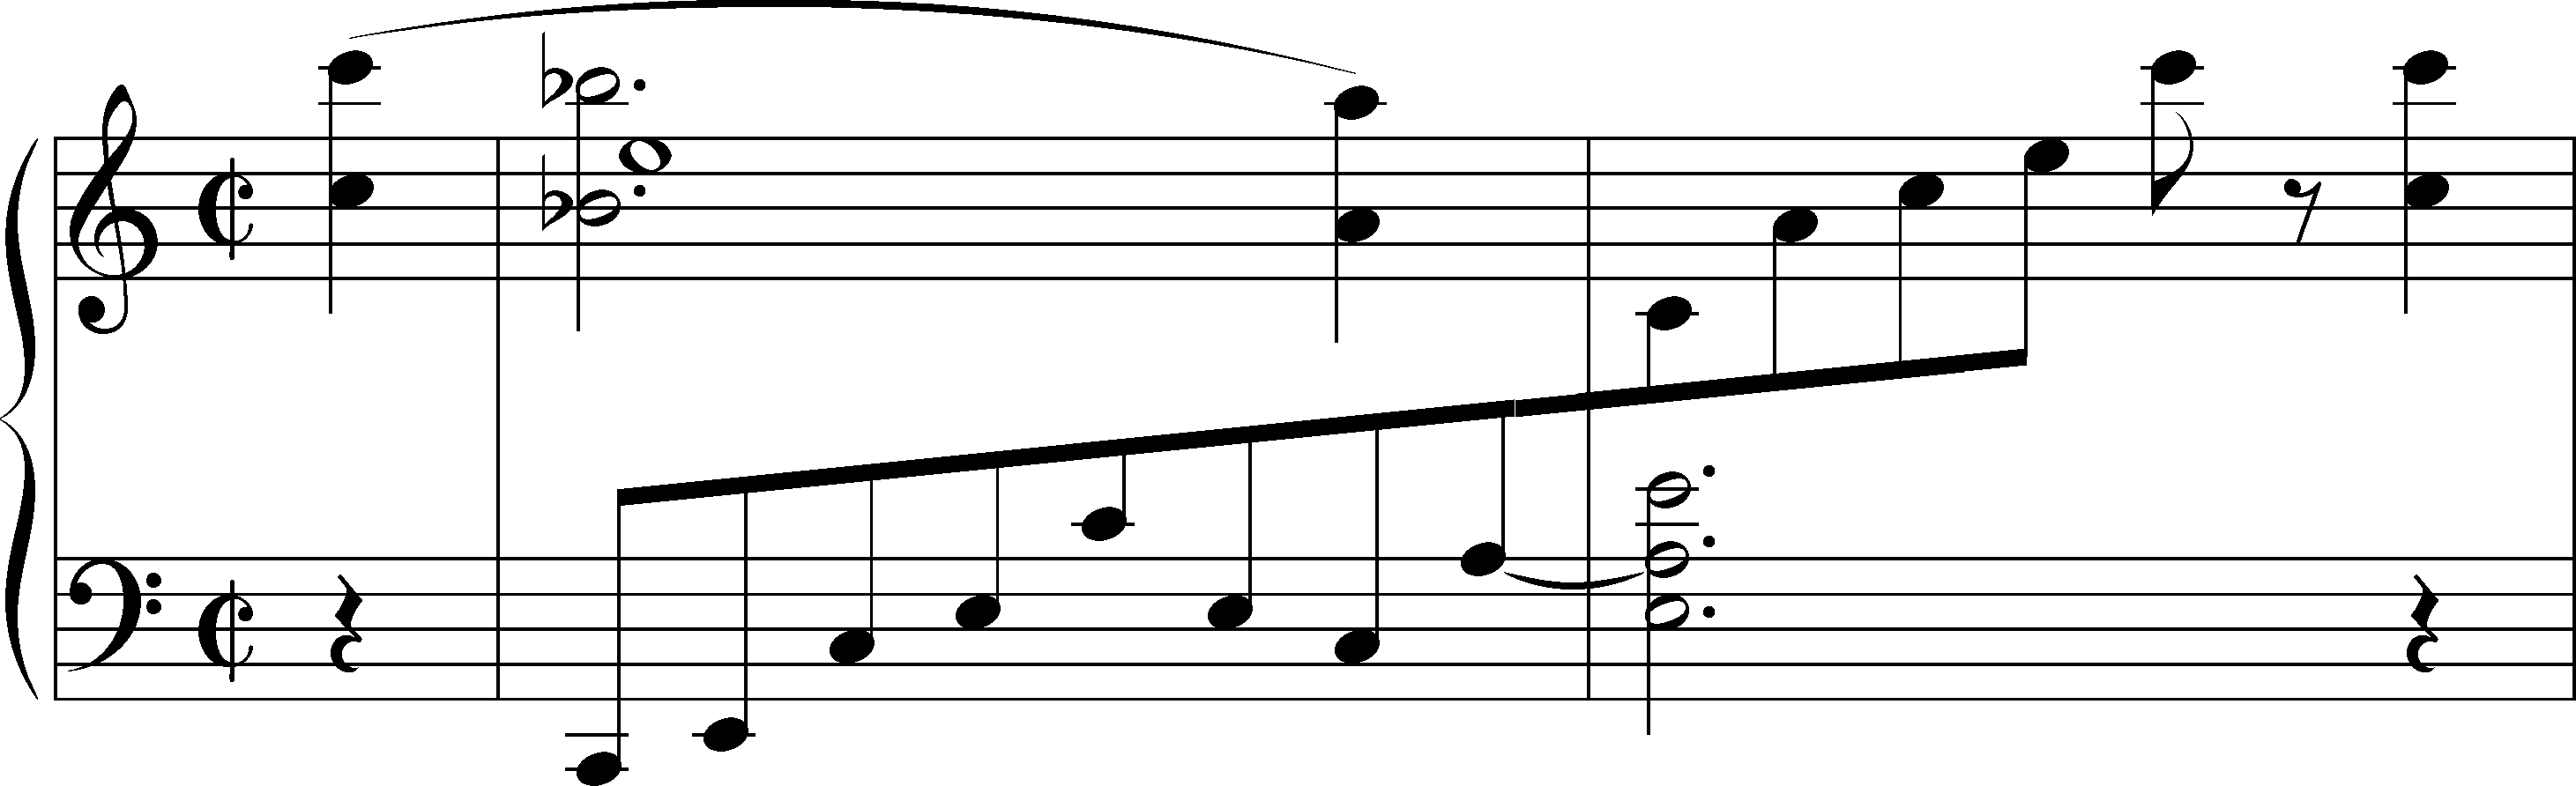
\includegraphics{musixtex}}
\end{center}

% FAQ: "Floats on their own on float pages"
% FAQ: "Vertical layout of float pages"
\begin{figure}[p]
  \centering
  \newcommand{\pagefigcapt}{Morbi justo at pretium eleifend diam}
  \faq{floatpages+vertposfp}%
    {"Floats on their own on float pages" and
     "Vertical layout of float pages"}%
    {\begin{minipage}{\widthof{Figure 99: \pagefigcapt}}
       \centering
       \usebox{\logobox} \\
       \caption{\pagefigcapt}
       \label{fig:1pagefig}
     \end{minipage}}
\end{figure}
\makeatletter
\afterpage{%
  \setlength{\@fptop}{0pt}
  \clearpage
  \setlength{\@fptop}{0pt plus 1fil}
}
\makeatother

% FAQ: "The comma as a decimal separator"
\newcommand*{\commafaq}[1]{%
  \faq{dec_comma}{"The comma as a decimal separator"}{#1\strut}%
}
Ne mel laoreet mentitum iudicabit, cum ut nullam sententi\ae{}, quis
splendide mea in. Ad his error tantas, eu per verear
$\commafaq{\ensuremath{5{,}784{,}365{,}343{,}410{,}709}} = 3 \times 11
\times 23 \times 113 \times \commafaq{\ensuremath{137{,}633}} \times
\commafaq{\ensuremath{490{,}019}}$ iracundia gubergren. Eu perpetua
consequuntur qui. Usu regione principes ea, ne semper definiebas est.
Mauris et enim in erat gravida fringilla. Mauris quis nibh. Morbi
volutpat in hac habitasse platea dictumst. Aliquam turpis leo, sodales
nec, gravida eu, feugiat dapibus, libero.  Quisque sed nulla id tellus
euismod consequat.

% FAQ: "Roman theorems"
\newtheorem{preromantheorem}{Theorem}
\newenvironment{romantheorem}[1][]{%
  \begin{preromantheorem}[#1]
  \upshape
}{%
  \end{preromantheorem}%
}
\bigskip
\noindent
\faq{theoremfmt}{"Roman theorems"}{%
\begin{minipage}{\linewidth}
  \begin{romantheorem}[Dolor commodo lobortis]
  \strut
  Phasellus cursus, turpis et consectetuer facilisis, magna nulla
  facilisis odio, quis tincidunt nisl est cursus massa. Pr\ae{}sent
  lacus velit, pharetra sit amet, rutrum sit amet, sollicitudin nec.
  \strut
  \end{romantheorem}
\end{minipage}
}

% FAQ: "Proof environment"
% FAQ: "Defining a new log-like function in LaTeX"
% FAQ: "Cancelling terms in maths expressions"
\begin{proof}
\renewcommand{\qed}{\quad\faq{proof}{"Proof
environment"}{\strut\rule{5pt}{5pt}}} Donec nunc turpis, scelerisque
in, sodales vit\ae{}, commodo et, sapien. Pellentesque elementum, orci
ut pulvinar posuere, pede velit convallis justo, at sodales risus
tellus ac lectus.  Pellentesque habitant morbi tristique senectus et
malesuada fames ac turpis egestas.
\begin{equation*}
\begin{array}[b]{rcl}
  \faq{newfunction}%
    {"Defining a new log-like function in LaTeX"}%
    {\ensuremath{\displaystyle\loremop_{p \in P}}}(x_p)
              &=& (x-1) (x+1) \\
              &=& [x \cdot 1 + (-1) \cdot 1] + [x \cdot x + (-1) \cdot x] \\
              &=& (x - 1) + (x^2 - x) \\
              &=& x^2 +
                  \faq{cancellation}{"Cancelling terms in maths expressions"}{%
                    \strut\ensuremath{\cancelto{0}{x - x}}\hspace*{1em}}
                  - 1 \\
              &=& x^2 - 1
\end{array}\tag*{\qedhere}
\end{equation*}
\end{proof}

Pr\ae{}sent a mauris. Quisque nunc tortor, commodo quis, consequat
eget elementum non eros.  \AE{}nean sollicitudin ipsum porttitor
nulla, donec dolor

\begin{equation}
\alpha \leq \int_m^{\log_2 m} K^{*}(z)\:\text{d}z < \beta \:,
\label{eq:repeatable}
\end{equation}

\noindent
fusce lectus elit.  Pellentesque ac tincidunt eget, pretium vel.
Vivamus mattis dui eget mauris. Proin varius. Cras ultrices suscipit
arcu. Nullam leo magna, faucibus nec, pulvinar eget, tempor et
sapien.

\bigskip

% FAQ: "Adjusting maths font sizes"
\noindent
\faq{mathsize}{"Adjusting maths font sizes"}{%
  \begin{minipage}{\linewidth}
  \fontsize{10.1}{12}\selectfont
  \begin{equation}
    \upsilon(t) = \frac{1+t^2}{1-\frac{2^t}{3t+5}}
  \end{equation}
  \end{minipage}
}

\bigskip

Cras ornare mauris sit amet ante vit\ae{} ante pretium
dignissim. Nulla facilisi, phasellus sapien enim, placerat id, posuere
eu, porta eget, risus. Quisque nisi pr\ae{}sent nibh urna, dapibus eu,
pretium vit\ae{} sollicitudin et nunc,

% FAQ: "Re-using an equation"
\begin{equation}
\alpha \leq \int_m^{\log_2 m} K^{*}(z)\:\text{d}z < \beta \:,
\tag{\faq{reuseq}{"Re-using an equation"}{\hypergetref{eq:repeatable}\strut}}
\end{equation}

\noindent
duis ultricies velit a justo gravida sagittis.  \AE{}nean bibendum
hendrerit ligula. Nam mattis pellentesque odio. Suspendisse ornare
aliquet tortor. Duis placerat euismod quam. Curabitur commodo volutpat
sem. Fusce enim tellus, congue a, luctus eget, tempus et, felis.

% FAQ: "Ellipses"
\newcommand*{\ellipsesfaq}[1]{\faq{mathlips}{"Ellipses"}{\ensuremath{#1}}}
\begin{equation}
\newcommand*{\fcdots}{\ellipsesfaq{\cdots}}
\newcommand*{\fvdots}{\ellipsesfaq{\vdots}}
\newcommand*{\fddots}{\ellipsesfaq{\ddots}}
\newcommand*{\fiddots}{\ellipsesfaq{%
  \mathinner{\mkern1mu\raise1pt
    \vbox{\kern7pt\hbox{.}}\mkern2mu
    \raise4pt\hbox{.}\mkern2mu\raise7pt\hbox{.}\mkern1mu}%
  }%
}
A^T
\left(
\begin{array}{ccccc}
1 & 2 & 3 & \fcdots & n \\
2 & 3 & 4 & \fcdots & n+1 \\
3 & 4 & 5 & \fcdots & n+2 \\
\fvdots & \fvdots & \fvdots & \fddots & \fvdots \\
n & n+1 & n+2 & \fcdots & 2n-1 \\
\end{array}
\right)
=
\left(
\begin{array}{ccccc}
\multicolumn{2}{c}{\text{\Huge 0}} & & & 1 \\
& & & \frac{1}{2} & \\
& & \frac{1}{3} & & \\
& \fiddots & & & \\
\frac{1}{n} & & & \multicolumn{2}{c}{\text{\Huge 0}} \\
\end{array}
\right)
\end{equation}

% FAQ: "Line-breaking in in-line maths"
Ornare mi convallis commodo et nulla, dapibus sollicitudin iaculis
diam curabitur aut volutpat, odio pellentesque sed posuere ipsum donec
lacinia. Adipiscing tellus dolor ut \antifaq{brkinline}{"Line-breaking
in in-line
maths"}{$a^3+$\strut}\linebreak[4]\antifaq{brkinline}{"Line-breaking
in in-line maths"}{$b=c$\strut}, tincidunt potenti urna sem phasellus
non nisl, nibh massa neque eget ac pellentesque cras. Nulla ac
adipiscing laoreet donec sit, pede quam duis ullamcorper lorem pede
molestie, blandit cras libero quis egestas id, id pulvinar in integer
vivamus vit\ae{} integer.

% FAQ: "Extra vertical space in floats"
% FAQ: "Automatic sizing of minipage"
% FAQ: "Spacing lines in tables"
\begin{table}[htp]
  \centering
  \antifaq{vertspacefloat}{"Extra vertical space in floats"}{\makebox[\linewidth]{\strut}}
  \begin{tabular}{|c|c|}
    \hline
    habitasse & condimentum \\ \hline
    \makebox[0pt]{\faq{struttab}{"Spacing lines in tables"}{\makebox[\wd\logobox+2\tabcolsep]{\strut}}} & \\
    \usebox{\logobox} & \raisebox{0.5\ht\logobox}[0pt][0pt]{pellentesque} \\ \hline
    caus\ae{} & delicatissimi \\ \hline
    tractatos & mediocritatem \\ \hline
    probo & \faq{varwidth}{"Automatic sizing of minipage"}{\parbox[t]{\widthof{mediocritatem}}{%
      Libris atqui cotidieque ac erroribus ei mucius deleniti
      ponderum.\strut}} \\ \hline
  \end{tabular}
  \caption{Pr\ae{}sent amet, ipsum leo scelerisque hac morbi libero}
  \label{tbl:extrarowheight}
  \antifaq{vertspacefloat}{"Extra vertical space in floats"}{\makebox[\linewidth]{\strut}}
\end{table}

Fusce id eros congue metus lacinia vit\ae{}, tortor posuere suscipit
convallis possimus cum nunc, commodo erat enim id tempor tortor, diam
id gravida quis lacinia leo volutpat, malesuada in eget ultrices
vit\ae{} volutpat aspernatur:

% FAQ: "Tables longer than a single page"
\newsavebox{\partialtabular}
\newcounter{romnum}
\begin{center}
\let\origminipage=\minipage
\let\origendminipage=\endminipage
\setlength{\columnwidth}{\widthof{99XXXVIII99000000}+8\tabcolsep+2em}
\newcommand{\dectorom}[1]{%
  \setcounter{romnum}{#1}%
  \MakeUppercase{\roman{romnum}}%
}
\renewenvironment{minipage}[1]{%
  \begin{lrbox}{\partialtabular}
  \origminipage{#1}%
}{%
  \origendminipage
  \end{lrbox}%
  \faq{longtab}{"Tables longer than a single page"}{\usebox{\partialtabular}}%
}
\let\topcapt=\STtopcapt
\begin{mpsupertabular}{|r|l|>{\ttfamily}r|r|}
  \hline
    1 & \dectorom{1}   & 01 & 000001 \\ \hline
    2 & \dectorom{2}   & 02 & 000010 \\ \hline
    3 & \dectorom{3}   & 03 & 000011 \\ \hline
    4 & \dectorom{4}   & 04 & 000100 \\ \hline
    5 & \dectorom{5}   & 05 & 000101 \\ \hline
    6 & \dectorom{6}   & 06 & 000110 \\ \hline
    7 & \dectorom{7}   & 07 & 000111 \\ \hline
    8 & \dectorom{8}   & 08 & 001000 \\ \hline
    9 & \dectorom{9}   & 09 & 001001 \\ \hline
   10 & \dectorom{10}  & 0A & 001010 \\ \hline
   11 & \dectorom{11}  & 0B & 001011 \\ \hline
   12 & \dectorom{12}  & 0C & 001100 \\ \hline
   13 & \dectorom{13}  & 0D & 001101 \\ \hline
   14 & \dectorom{14}  & 0E & 001110 \\ \hline
   15 & \dectorom{15}  & 0F & 001111 \\ \hline
   16 & \dectorom{16}  & 10 & 010000 \\ \hline
   17 & \dectorom{17}  & 11 & 010001 \\ \hline
   18 & \dectorom{18}  & 12 & 010010 \\ \hline
   19 & \dectorom{19}  & 13 & 010011 \\ \hline
   20 & \dectorom{20}  & 14 & 010100 \\ \hline
   21 & \dectorom{21}  & 15 & 010101 \\ \hline
   22 & \dectorom{22}  & 16 & 010110 \\ \hline
   23 & \dectorom{23}  & 17 & 010111 \\ \hline
   24 & \dectorom{24}  & 18 & 011000 \\ \hline
   25 & \dectorom{25}  & 19 & 011001 \\ \hline
   26 & \dectorom{26}  & 1A & 011010 \\ \hline
   27 & \dectorom{27}  & 1B & 011011 \\ \hline
   28 & \dectorom{28}  & 1C & 011100 \\ \hline
   29 & \dectorom{29}  & 1D & 011101 \\ \hline
   30 & \dectorom{30}  & 1E & 011110 \\ \hline
   31 & \dectorom{31}  & 1F & 011111 \\ \hline
   32 & \dectorom{32}  & 20 & 100000 \\ \hline
   33 & \dectorom{33}  & 21 & 100001 \\ \hline
   34 & \dectorom{34}  & 22 & 100010 \\ \hline
   35 & \dectorom{35}  & 23 & 100011 \\ \hline
   36 & \dectorom{36}  & 24 & 100100 \\ \hline
   37 & \dectorom{37}  & 25 & 100101 \\ \hline
   38 & \dectorom{38}  & 26 & 100110 \\ \hline
   39 & \dectorom{39}  & 27 & 100111 \\ \hline
   40 & \dectorom{40}  & 28 & 101000 \\ \hline
   41 & \dectorom{41}  & 29 & 101001 \\ \hline
   42 & \dectorom{42}  & 2A & 101010 \\ \hline
   43 & \dectorom{43}  & 2B & 101011 \\ \hline
   44 & \dectorom{44}  & 2C & 101100 \\ \hline
   45 & \dectorom{45}  & 2D & 101101 \\ \hline
   46 & \dectorom{46}  & 2E & 101110 \\ \hline
   47 & \dectorom{47}  & 2F & 101111 \\ \hline
   48 & \dectorom{48}  & 30 & 110000 \\ \hline
   49 & \dectorom{49}  & 31 & 110001 \\ \hline
   50 & \dectorom{50}  & 32 & 110010 \\ \hline
\end{mpsupertabular}
\end{center}

% FAQ: "My words aren't being hyphenated"
% FAQ: "Hyphenation exceptions"
% FAQ: "Weird hyphenation of words"
% FAQ: "(Merely) peculiar hyphenation"
Ullamcorper penatibus morbi nulla arcu luctus, phasellus nullam
consequat quam fusce curabitur, auctor integer felis neque
\antifaq{nohyph+hyphexcept}{"My words aren't being hyphenated" and
"Hyphenation
exceptions"}{e\=osvider\'erap\v{e}iriann\H{o}anviserr\"oriuvareti\d{u}stopl\r{a}cerat\ss{}imiliquem\b{e}iexpr\oe{}pi\c{c}uri\^eff\`{\i}ciendi\strut}
turpis ad at, malesuada ante lacinia quis ante vehicula, arcu pulvinar
aliquam in eros.  Reque gr\ae{}co volutpat at eum. Et etiam falli
omittam nec, ludus nostro delicata cu sit. Ut autem oportere sit. Duo
malis adipisci id, id per omnium takimata repudiand\ae{}. Ex cum
\antifaq{weirdhyphen+oddhyphen}{"Weird hyphenation of words" and
"(Merely) peculiar
hyphenation"}{n-\strut}\linebreak[4]\antifaq{weirdhyphen+oddhyphen}{"Weird
hyphenation of words" and "(Merely) peculiar hyphenation"}{ibh\strut}
augue epicuri.  Percipit invenire mediocrem ad mel, eu agam atqui
mei. Vis ei vocent urbanitas duis nominati honestatis vel.
Pellentesque sollicitudin urna eget nulla. Nulla imperdiet
sollicitudin leo. Phasellus odio. Nam scelerisque dolor ut mi.

% FAQ: "How to alter the alignment of tabular cells"
% FAQ: "How to change a whole row of a table"
\begin{table}[tbp]
  \centering
  \begin{tabular}{|l|l|p{12pc}|}
  \hline
  sagittis & faucibus &
  Natoque ut consectetuer vel consequatur pulvinar ultricies, justo
  duis venenatis suspendisse risus tincidunt nec, rhoncus lorem et ut
  consequat eu sed, a nulla lacus ut felis mi pellentesque. \\ \hline

  \itshape \textcolor{blue}{porta} &
  \itshape \textcolor{blue}{justo} &
  \itshape \textcolor{blue}{Etiam tellus lectus nulla vit\ae{}.}\strut \\ \hline
  \noalign{\smash{%
    \raisebox{3pt}{\faq{wholerow}{"How to change a whole row of a table"}{%
      \strut
      \rule{12pc+6\tabcolsep+\widthof{sagittis}+\widthof{ac mauris}}{0pt}%
    }}%
  }}

  quam     & ac mauris  &
  Amet cursus nunc pellentesque imperdiet pellentesque vel, convallis
  purus aliquam hac condimentum duis vel, sit mollitia lorem id a arcu
  at massa leo. \\ \hline

  nulla    & pede       &
  \strut
  \faq{tabcellalign}{"How to alter the alignment of tabular cells"}{%
    \begin{minipage}[t]{\linewidth}
      \centering\strut
      Wisi magnis \AE{}nean ante parturient nec felis, sem vel arcu
      vestibulum justo fugit, proin laoreet possimus \AE{}nean iaculis
      at metus.\strut
    \end{minipage}%
  } \\ \hline
  \end{tabular}
  \caption{Pretium vivamus accumsan}
  \label{tbl:centercell}
\end{table}

% FAQ: "The thickness of rules in LaTeX tables"
\begin{table}[tbp]
  \centering
  \setlength{\arrayrulewidth}{3pt}
  \faq{rulethk}{"The thickness of rules in LaTeX tables"}{%
    \begin{tabular}{|c|c|c|c|}
    \hline
     odio    & vestibulum & ligula   & porta       \\ \hline
     tortor  & rhoncus    & montes   & fermentum   \\ \hline
     commodo & nulla      & interdum & scelerisque \\ \hline
    \end{tabular}%
  }
  \caption{Amet fusce turpis sapien ac eleifend hac}
  \label{tbl:thicklines}
\end{table}

% FAQ: "Preventing hyphenation of a particular word"
% FAQ: "Stopping all hyphenation"
Vel eu modus simul iriure, mei cu unum nominavi, eos postea
\faq{wdnohyph+hyphoff}{"Preventing hyphenation of a particular word"
and "Stopping all
hyphenation"}{delicatissimietveniameleifendintellegameamubiqueoportereargumentumetvix\strut}
facer movet usu ne, facilis qualisque ne mei. Decore gr\ae{}cis
verterem at qui. An ceteros voluptua consectetuer sed, te ius accumsan
posidonium, pro ei quis principes.

% FAQ: "Version control using RCS, CVS or Subversion"
\begin{center}
\faq{RCS}%
  {"Version control using RCS, CVS or Subversion"}%
  {\texttt{\$Id:~visfaq.tex,v 1.00 2006/02/12 17:06:31 pakin Exp \$}}
\end{center}

\clearpage

% FAQ: "How to change LaTeX's 'fixed names'"
\renewcommand{\refname}{Voluptatibus}
\let\origthebibliography=\thebibliography
\makeatletter
\renewenvironment{thebibliography}[1]
     {\section*{\faq{fixnam}{"How to change LaTeX's 'fixed names'"}{\refname}}%
      \@mkboth{\MakeUppercase\refname}{\MakeUppercase\refname}%
      \list{\@biblabel{\@arabic\c@enumiv}}%
           {\settowidth\labelwidth{\@biblabel{#1}}%
            \leftmargin\labelwidth
            \advance\leftmargin\labelsep
            \@openbib@code
            \usecounter{enumiv}%
            \let\p@enumiv\@empty
            \renewcommand\theenumiv{\@arabic\c@enumiv}}%
      \sloppy
      \clubpenalty4000
      \@clubpenalty \clubpenalty
      \widowpenalty4000%
      \sfcode`\.\@m}
     {\def\@noitemerr
       {\@latex@warning{Empty `thebibliography' environment}}%
      \endlist}
\makeatother

\begin{thebibliography}{9}
% FAQ: "Accents in bibliographies"
\bibitem{accents}
Numquam Deserunt.
\newblock Minimum \faq{bibaccent}{"Accents in
bibliographies"}{r\'e\c{c}\"us\`ab\H{o}} salutandi pro cu.
\newblock In \emph{Ei Usu Inermis Veritus Evertitur}, 1995.

% FAQ: "Format of numbers in the bibliography"
\makeatletter
\let\orig@biblabel=\@biblabel
\renewcommand*{\@biblabel}[1]{%
  \faq{formbiblabel}{"Format of numbers in the bibliography"}{\hfill#1.\strut}%
}
\bibitem{format-numbers}
Choro Fabellas, Modus Consetetur, and Homero D. Invenire.
\newblock Iudico oratio ea sed: Nibh legendos quo an.
\newblock Technical Report~DXVII, University of Iracundia, August 1979.
\let\@biblabel=\orig@biblabel
\makeatother

% FAQ: "Capitalisation in BibTeX"
\newcommand*{\captitlefaq}[1]{%
  \faq{capbibtex}{"Capitalisation in BibTeX"}{#1\strut}%
}
\bibitem{cap-title}
Duis Indoctum and Primis Qu\ae{}stio.
\newblock \captitlefaq{P}er \captitlefaq{I}d,
  \captitlefaq{M}ei \captitlefaq{N}o \captitlefaq{A}utem.
\newblock \emph{Vituperata Signiferumque}, 7(12), December 1981.

% FAQ: "Transcribed initials in BibTeX"
\bibitem{initials}
\faq{bibtranscinit}{"Transcribed initials in BibTeX"}{Yu.\strut} Iriure and
\faq{bibtranscinit}{"Transcribed initials in BibTeX"}{Ya.\strut} Porrov.
\newblock Mei recteque: Sententi\ae{} ad error essent.
\newblock \emph{Meis Iriure Molesti\ae}, volume~25, Winter~2001.

% FAQ: "References from the bibliography to the citation"
\bibitem{backref}\label{cite:backref}
Ridens Laboramus, Congue Nominati Adolescens, Quidam S. Constituto,
  and Ullum Honestatis.
\newblock \emph{Inani Melius Nam Ad---Pri ei Facete Dissentiunt}.
\newblock Ferri Prompta version~3.1, October 2005.
\newblock \faq{backref}{"References from the bibliography to the
  citation"}{Pages~\hypergetpageref{backbackref1},
  \hypergetpageref{backbackref2}, \hypergetpageref{backbackref3}}.

% FAQ: "Non-english bibliographies"
\newcommand{\foreign}[1]{%
  \faq{i18nbib}{"Non-english bibliographies"}{\usefont{U}{psy}{m}{n}#1\strut}%
}
\bibitem{non-english}
Congue Magna, Duo Cu, \foreign{and} Mucius Veritus.
\newblock Oblique definiebas.
\newblock \foreign{In} Aliquip Laoreet \foreign{and} Gr\ae{}ci Dicunt,
  \foreign{editors}, \emph{Ne Sea Patrioque an Mei},
  \foreign{number}~35 \foreign{in} Facilis Contentiones,
  \foreign{part}~2, \foreign{pages}~189--201, Has Consectetuer, Ut
  Esse, 3rd~\foreign{edition}, \foreign{November}~1986.

% FAQ: "Choosing a bibliography style"
\makeatletter
\let\orig@biblabel=\@biblabel
\renewcommand*{\@biblabel}[1]{%
  [\faq{whatbst}{"Choosing a bibliography style"}{Dapibus, 1938\strut}]%
}
\bibitem{whatbst}
Morbi Dapibus,
\newblock Cum sociis natoque penatibus et magnis dis parturient montes,
\newblock In \emph{Proc.\ of the 8th Intl.\ Conf.\ on Vestibulum Tincidunt},
\newblock Jan. 3, 1938.

Choro Fabellas, Modus Consetetur, and Homero D. Invenire.
\newblock Iudico oratio ea sed: Nibh legendos quo an.
\newblock Technical Report~DXVII, University of Iracundia, August 1979.
\let\@biblabel=\orig@biblabel
\makeatother

% FAQ: "Multiple citations"
\bibitem{multicite}
\faq{mcite}{"Multiple citations"}{\parbox[t]{\linewidth}{%
Paulo Omittam, Vocent A. Fugit, Mentitum Ponderum, and Vero Lorem
Mediocritatem,
\newblock Qu\ae{}rendum et Sit~\textbf{13} (1954);
\newblock Munere Detraxit and Soleat Epicurei,
\newblock in: Pro Torquatos~(ed.),
\newblock \emph{Intellegebat ea Rebum}, p.~121, Nullam Iriure, 1966;
\newblock Sumo Detraxit,
\newblock Sonet Inimicus Hendrerit~\textbf{31} (1972)~1126.}}

% FAQ: "Creating a bibliography style"
\bibitem{custbib}
\faq{custbib}{"Creating a bibliography style"}{\parbox[t]{\linewidth}{\strut
  Platonem,~F, JR Cotidieque, C~Dolore, et al.~(1979).
  \newblock \uline{Sint Laoreet Scriptorem},
  \newblock In: \emph{J.~Moll Erip Disputando},
  \newblock Vol.~3, No.~15 (January), pp.~112-135.
  \newblock ISBN:~0130388858; DOI:~10.1007/b99409,
  URL:~\nolinkurl{http://www.pakin.org/~scott}.}}

% FAQ: "BibTeX sorting and name prefixes"
\bibitem{name-prefix}
\faq{bibprefixsort}%
  {"BibTeX sorting and name prefixes"}%
  {Lord Recteque},
P. Aperiam, and S. Sensibus.
\newblock Per debet aperiri urbanitas ne.
\newblock In \emph{Sit at Soleat Nullam Gr\ae{}ci}, April--May, 1997.

% FAQ: "Reducing spacing in the bibliography"
\vspace*{-3ex}%
\faq{compactbib}%
  {"Reducing spacing in the bibliography"}%
  {\rule{\linewidth}{0pt}}%
\vspace*{-3ex}%

% FAQ: "URLs in BibTeX bibliographies"
\bibitem{normal}
Agam Prima,  Congue Everti, and Appetere Facilisis.
\newblock Suas eros melius id mel.
\newblock \emph{Altera Moderatius}, 66(7):55--68, July 2002.
\newblock Te soleat percipitur an sit ne
  \faq{citeURL}%
    {"URLs in BibTeX bibliographies"}%
    {\nolinkurl{http://www.ctan.org/tex-archive/info/visualFAQ/}}

% FAQ: "URLs in BibTeX bibliographies"
\bibitem{urls}
\faq{citeURL}%
  {"URLs in BibTeX bibliographies"}%
  {\nolinkurl{http://www.ctan.org/tex-archive/info/visualFAQ/}}
\end{thebibliography}

\bigskip

% FAQ: "Multiple bibliographies?"
\let\thebibliography=\origthebibliography
\noindent
\faq{multbib}{"Multiple bibliographies?"}{%
  \begin{minipage}{\linewidth}
  \renewcommand{\refname}{Voluptatibus~II}
  \begin{thebibliography}{Con01}
  \bibitem[Con01]{normal2}
  Te Consetetur.
  \newblock \emph{Dissentiunt Conclusionemque ne cum Nullam
  Vituperata: An Mollis Vivendo Maluisset cum ea Quod Eripuit
  Indoctum}.
  \newblock {PhD} dissertation, Vulputate University, August 2001.

  \bibitem[PR73]{normal1}
  Detraxit Pertinax and Nisl Regione.
  \newblock \emph{Elitr Invidunt Referrentur}.
  \newblock Placerat Singulis Scriptorem, Atqui, Vivendum, 2nd ed.,
    March 1973.
  \end{thebibliography}
  \end{minipage}
}

\bigskip

\appendix

\section{Fringilla dictum hendrerit}

Integre nusquam percipitur ad nec, ius viderer nostrud reformidans
ex. Hinc reque assentior eu nam, usu ea duis facilis. Cetero
forensibus sed ne, qui ei recteque tractatos. Quis mazim gr\ae{}co vis
ne. Vel et labitur comprehensam. Risus ac nibh nisl ultrices minus
facilisis, cum rhoncus tristique urna blandit magnis lobortis, eget
integer justo culpa lacus aliquet.

% FAQ: "All the files used by this document"
\newsavebox{\filelistapdx}
\begin{lrbox}{\filelistapdx}
\begin{minipage}{\linewidth}
\begin{multicols}{2}
\begin{Verbatim}[fontsize=\tiny]
 *File List*
 article.cls    2001/04/21 v1.4e Standard LaTeX document class
  size10.clo    2001/04/21 v1.4e Standard LaTeX file (size option)
    etex.sty    1998/03/26 v2.0 eTeX basic definition package (PEB)
geometry.sty    2002/07/08 v3.2 Page Geometry
  keyval.sty    1999/03/16 v1.13 key=value parser (DPC)
geometry.cfg    2001/06/05 v1.0 teTeX (uncustomised setup)
fancyhdr.sty
lastpage.sty    1994/06/25 v0.1b LaTeX2e package for refs to last page number (
JPG)
lettrine.sty    2002/10/26 v1.4 (D. Flipo)
lettrine.cfg
 type1cm.sty    2002/09/05 v0.04 BlueSky/Y&Y Type1 CM font definitions (DPC, pa
tched RF)
tabularx.sty    1999/01/07 v2.07 `tabularx' package (DPC)
   array.sty    1998/05/13 v2.3m Tabular extension package (FMi)
textcomp.sty    2001/06/05 v1.94 Standard LaTeX package
  ts1enc.def    2001/06/05 v3.0e (jk/car/fm) Standard LaTeX file
supertabular.sty    2002/07/19 v4.1e the supertabular environment
 topcapt.sty    2004/12/11 v1.2 Caption at top of float
graphicx.sty    1999/02/16 v1.0f Enhanced LaTeX Graphics (DPC,SPQR)
graphics.sty    2001/07/07 v1.0n Standard LaTeX Graphics (DPC,SPQR)
    trig.sty    1999/03/16 v1.09 sin cos tan (DPC)
graphics.cfg    2001/08/31 v1.1 graphics configuration of teTeX/TeXLive
  pdftex.def    2002/06/19 v0.03k graphics/color for pdftex
   color.sty    1999/02/16 v1.0i Standard LaTeX Color (DPC)
   color.cfg    2001/08/31 v1.1 color configuration of teTeX/TeXLive
  layout.sty    2000/09/25 v1.2c Show layout parameters
setspace.sty    2000/12/01 6.7 Contributed and Supported LaTeX2e package
 wrapfig.sty    2003/01/31  v 3.6
 amsmath.sty    2000/07/18 v2.13 AMS math features
 amstext.sty    2000/06/29 v2.01
  amsgen.sty    1999/11/30 v2.0
  amsbsy.sty    1999/11/29 v1.2d
  amsopn.sty    1999/12/14 v2.01 operator names
 amssymb.sty    2002/01/22 v2.2d
amsfonts.sty    2001/10/25 v2.2f
mathrsfs.sty    1996/01/01 Math RSFS package v1.0 (jk)
texnames.sty
bold-extra.sty    2001/11/13 v0.1 Use fonts from cm/mf-extra/bold
 eurosym.sty    1998/08/06 v1.1 European currency symbol ``Euro''
slashbox.sty
multirow.sty
afterpage.sty    1995/10/27 v1.08 After-Page Package (DPC)
 eso-pic.sty    2002/11/16 v1.1b eso-pic (RN)
everyshi.sty    2001/05/15 v3.00 EveryShipout Package (MS)
    calc.sty    1998/07/07 v4.1b Infix arithmetic (KKT,FJ)
multicol.sty    2000/07/10 v1.5z multicolumn formatting (FMi)
rotating.sty    1997/09/26, v2.13 Rotation package
  ifthen.sty    2001/05/26 v1.1c Standard LaTeX ifthen package (DPC)
fancyvrb.sty    2000/03/21
 makeidx.sty    2000/03/29 v1.0m Standard LaTeX package
  framed.sty    2002/12/29 v 0.5: framed or shaded text with page breaks
  cancel.sty    2000/03/12 v2.1 Cancel math terms
  amsthm.sty    2000/10/26 v2.08
    ulem.sty    2000/05/26
hyperref.sty    2003/01/22 v6.73n Hypertext links for LaTeX
  pd1enc.def    2003/01/22 v6.73n Hyperref: PDFDocEncoding definition (HO)
hyperref.cfg    2002/06/06 v1.2 hyperref configuration of TeXLive and teTeX
     url.sty    1999/03/28  ver 1.5x  Verb mode for urls, etc.
 hpdftex.def    2003/01/22 v6.73n Hyperref driver for pdfTeX
  pifont.sty    2002/09/08 PSNFSS-v9.0a Pi font support (SPQR)
    upzd.fd    2001/06/04 font definitions for U/pzd.
    upsy.fd    2001/06/04 font definitions for U/psy.
lorem-ipsum-logo.png    Graphic file (type png)
  ts1cmr.fd    1999/05/25 v2.5h Standard LaTeX font definitions
supp-pdf.tex
 nameref.sty    2001/01/27 v2.19 Cross-referencing by name of section
  visfaq.out
  ot1phv.fd    2001/06/04 scalable font definitions for OT1/phv.
   ursfs.fd    1998/03/24 rsfs font definition file (jk)
  ot1pnc.fd    2001/06/04 font definitions for OT1/pnc.
 ts1cmtt.fd    1999/05/25 v2.5h Standard LaTeX font definitions
   t1pzc.fd    2001/06/04 font definitions for T1/pzc.
fuzzytext.png    Graphic file (type png)
   t1ptm.fd    2001/06/04 font definitions for T1/ptm.
   t1phv.fd    2001/06/04 scalable font definitions for T1/phv.
   t1pcr.fd    2001/06/04 font definitions for T1/pcr.
   t1pag.fd    2001/06/04 font definitions for T1/pag.
   t1pbk.fd    2001/06/04 font definitions for T1/pbk.
   t1ppl.fd    2001/06/04 font definitions for T1/ppl.
   t1pnc.fd    2001/06/04 font definitions for T1/pnc.
   t1bch.fd    2001/06/04 font definitions for T1/bch.
visfaq-html.png    Graphic file (type png)
  t1cmss.fd    1999/05/25 v2.5h Standard LaTeX font definitions
watermark.pdf    Graphic file (type pdf)
book-montage.png    Graphic file (type png)
labelgraph.pdf    Graphic file (type pdf)
musixtex.png    Graphic file (type png)
  visfaq.ind
  visfaq.ind2
anotherarticle.pdf    Graphic file (type pdf)
 ***********
\end{Verbatim}
\end{multicols}
\end{minipage}
\end{lrbox}
\noindent
\faq{filesused}%
  {"All the files used by this document"}%
  {\usebox{\filelistapdx}\strut}

\bigskip

Dolores reformidans in cum, vim recteque aliquando no. Ne veri laudem
vis, ludus dicunt at vix. Dico inani ut vim. Nam an summo volumus
constituto, qui te \ae{}que petentium. At odio ludus voluptua pri, no
essent lucilius eum.

\bigskip

% FAQ: "Appendixes"
% FAQ: "Balancing columns at the end of a document"
%\noindent
%\begin{minipage}{\linewidth}
\begin{multicols}{2}
\newcommand{\appendixBname}{Ubique nunc facilis mollis gubergren}
\section*{\faq{appendix}{"Appendixes"}{%
  Appendix~B}\quad\raggedright\appendixBname}
\sectionmark{\appendixBname}
\phantomsection
\addcontentsline{toc}{section}{\appendixBname}

Ornare eleifend. Dictum pr\ae{}sent quisque pretium hac consequat
lobortis taciti pulvinar amet volutpat nascetur at pellentesque
nascetur ut. Molestie congue, eu porttitor egestas blandit pharetra
conubia suspendisse fermentum hac vit\ae{} nunc mollis platea
in. Mauris primis ullamcorper. Tristique, semper sodales.
Ridiculus pharetra vivamus fames rutrum. Ac habitant phasellus. Wisi
magnis dictum nunc \ae{}nean tellus ad facilisi ultricies molestie
adipiscing sociis sagittis scelerisque proin non. Vivamus interdum
venenatis velit posuere. Potenti quis nascetur in. In imperdiet, ipsum
semper.

Proin natoque primis natoque, habitasse mi facilisis velit cur\ae{}
netus ut. Tincidunt etiam facilisi commodo volutpat. Id varius lacus,
rhoncus fermentum iaculis rutrum primis dictumst semper lectus
ultrices id. Proin platea rutrum. Hymen\ae{}os nullam, justo
ultrices. Dui nonummy, phasellus eros est aptent dis. Mauris, arcu non
elit.  Phasellus cursus scelerisque. Molestie mollis. Imperdiet sem
sodales scelerisque pretium habitant magnis. Diam dis. In ullamcorper
ante. Pede cum. Sociis imperdiet taciti.

Gravida nonummy. Pede donec accumsan porttitor curabitur. Fames, et
curabitur velit augue rhoncus fames m\ae{}cenas orci tempor laoreet
lorem consectetuer lobortis ut massa. Laoreet cursus. Sem sociosqu
platea ad. Diam vehicula. Duis blandit.  Suscipit proin rutrum magna
nonummy dui venenatis. Torquent, egestas nunc eu. Accumsan platea, non
suscipit imperdiet. Ridiculus, sapien ornare posuere est. Porta
cur\ae{}. Varius cras aliquam curabitur class. Volutpat, volutpat
litora est.  Quisque sit amet urna quis mauris porta fermentum.
Quisque lectus mauris, porttitor eu, dignissim quis, vulputate a metus
suspendisse aliquam.

Eu fusce sollicitudin cras pr\ae{}sent. Magna erat m\ae{}cenas dis, mi
gravida vulputate. Orci pede lectus. Nibh, tellus libero
lacinia. Tempus consequat. Interdum interdum vit\ae{} montes consequat
lectus id nostra porta suspendisse sem duis. Lectus, porttitor lectus.
\end{multicols}
\noindent
\raisebox{4ex}[0pt][0pt]{%
  \makebox[\linewidth]{%
    \faq{balance}{"Balancing columns at the end of a document"}{%
      \rule{\linewidth+1cm}{0pt}%
      \rule{0pt}{2\baselineskip}%
    }%
  }%
}
%\end{minipage}

% FAQ: "How to ask a question"
% FAQ: "How to make a 'minimum example'"
\begin{figure}[bp]
  \centering
  \setlength{\unitlength}{1pt}
  \faq{askquestion+minxampl}%
    {"How to ask a question" and "How to make a 'minimum example'"}%
    {\scalebox{2}{%
       \begin{picture}(100,100)
         \color{blue}
         \fontsize{100}{100}\usefont{OT1}{pbk}{bx}{n}
         \put(15,15){?}
         \color[rgb]{0.5,0,0.5}
         \fontsize{40}{40}\usefont{OT1}{pag}{bx}{n}
         \put(0,0){?}
         \put(0,70){?}
         \put(80,0){?}
         \put(80,70){?}
         \color[rgb]{1,0.5,0}
         \fontsize{20}{20}\usefont{OT1}{pzc}{m}{it}
         \put(50,0){?}
         \put(50,87){?}
         \put(0,45){?}
         \put(90,45){?}
       \end{picture}%
     }%
    }
\end{figure}

% FAQ: "Generating an index in (La)TeX"
\bigskip
\makeatletter
\newif\ifscan@allowed
\def\dotfill{\leaders\hbox to.6em{\hss .\hss}\hskip\z@ plus 1fill}%
\def\dotfil{\leaders\hbox to.6em{\hss .\hss}\hfil}%
\def\pfill{\unskip~\dotfill\penalty500\strut\nobreak
           \dotfil~\ignorespaces}%
\makeatother
\noindent
\faq{makeindex}{"Generating an index in (La)TeX"}{%
  \begin{minipage}{\linewidth}
    \printindex
  \end{minipage}%
}

\null\vskip 3.5ex plus -1ex minus -.2ex\null

% FAQ: "Multiple indexes"
\noindent
\faq{multind}{"Multiple indexes"}{%
  \begin{minipage}{\linewidth}
    \input{\jobname.ind2}
  \end{minipage}%
}

% FAQ: "A 'report' from lots of 'article's"
\clearpage
\null
\thispagestyle{empty}
\centergraphic*{anotherarticle}
\AddToShipoutPicture*{%
  \put(0,0){%
    \faq{multidoc}%
      {"A 'report' from lots of 'article's"}%
      {\rule{0pt}{\paperheight}\rule{\paperwidth}{0pt}}}
}

% FAQ: "Moving tables and figures in LaTeX"
\begin{figure}[p]
  \centering
  \antifaq{floats}{"Moving tables and figures in LaTeX"}{\usebox{\logobox}}
  \caption{Nusquam probatus expetenda}
  \label{fig:endfloat-bad}
\end{figure}
\begin{figure}[p]
  \centering
  \faq{floats}{"Moving tables and figures in LaTeX"}{\usebox{\logobox}}
  \caption{Tale omittantur eum}
  \label{fig:endfloat-good}
\end{figure}

\end{document}
